\documentclass[conference]{IEEEtran}
\IEEEoverridecommandlockouts

\usepackage{amsmath,amssymb,amsfonts}
\usepackage{algorithmic}
\usepackage{graphicx}
\usepackage{textcomp}
\usepackage{xcolor}
\usepackage{booktabs}
\usepackage{multirow}
\usepackage{cite}
\usepackage{url}
\usepackage{microtype}
\usepackage[hidelinks]{hyperref}
\hypersetup{
    pdftitle={Graph Neural Networks versus Tabular Machine Learning for Illicit Transaction Detection in Bitcoin: An Empirical Evaluation under Chronological Partitioning},
    pdfauthor={Khushi},
    pdfsubject={Blockchain Forensics and Graph Neural Networks},
    pdfkeywords={Bitcoin, illicit transaction detection, fraud detection, graph neural networks, GraphSAGE, GCN, GAT, tabular machine learning, temporal generalization, class imbalance}
}


\def\BibTeX{{\rm B\kern-.05em{\sc i\kern-.025em b}\kern-.08em
    T\kern-.1667em\lower.7ex\hbox{E}\kern-.125emX}}

\begin{document}

\title{Graph Neural Networks versus Tabular Machine Learning for Illicit Transaction Detection in Bitcoin: An Empirical Evaluation under Chronological Partitioning}

\author{\IEEEauthorblockN{Khushi}
\IEEEauthorblockA{\textit{Department of Artificial Intelligence and Data Science} \\
\textit{Indira Gandhi Delhi Technical University for Women} \\
Delhi, India \\
khushi086btcseai23@igdtuw.ac.in}
}

\maketitle

\begin{abstract}
The detection of illicit transactions in public cryptocurrency ledgers is a critical challenge in financial forensic technology and regulatory compliance. Graph Neural Networks (GNNs) have emerged as an intuitive paradigm for blockchain analysis, operating on the premise that topological message passing over transaction networks will outperform conventional machine learning models. However, past empirical benchmarks frequently employ random cross-validation or feature-rich baselines that obscure the isolated inductive benefit of graph structure. In this work, we present a rigorous, reproducible empirical comparison between three foundational Graph Neural Network architectures (GCN, GraphSAGE, GAT) and four strong conventional machine learning baselines (Logistic Regression, Random Forest, XGBoost, MLP) using the Elliptic Bitcoin benchmark under a strict chronological evaluation protocol ($T = 49$ time steps). Our experimental design controls for feature representations ($93$ local features vs. $165$ full features), class-imbalance loss formulations (standard vs. cost-sensitive weighted cross-entropy), and multi-seed parameter initialization ($N = 5$ random seeds). Across the full 165-dimensional feature space, conventional tree-based ensembles demonstrate strong performance, with Random Forest achieving a holdout test illicit F1-score of $0.7247 \pm 0.0027$ (PR-AUC $0.6599 \pm 0.0025$) and XGBoost achieving $0.7131 \pm 0.0111$ (PR-AUC $0.6744 \pm 0.0028$), compared to $0.3308 \pm 0.0602$ for GAT, $0.2822 \pm 0.1248$ for GraphSAGE, and $0.2589 \pm 0.0639$ for GCN. We observe that tabular models benefit consistently from pre-engineered 1-hop aggregate features ($\Delta\text{F1} = +0.0311$ to $+0.0430$), whereas GNN sensitivity to feature representation is architecture-dependent. Furthermore, extensive ablation studies reveal that GNN performance is highly sensitive to graph directionality, unknown-node topological context, and random initialization seed variance (GCN F1 range $0.4686$; GraphSAGE F1 range $0.3669$). Statistical comparisons between the validation-selected GNN (GraphSAGE on local features, test F1 $0.4153 \pm 0.1914$) and tree baselines yield raw paired $t$-test differences ($p \approx 0.023$) that do not remain statistically significant following Holm-Bonferroni correction ($p_{\text{Holm}} = 0.0917$) or exact Wilcoxon signed-rank testing ($p = 0.0625$), bounded by small sample power limits ($N=5$). All models exhibit substantial temporal generalization degradation (relative F1 drops of $23.6\%$ to $44.9\%$) across chronological splits, driven by marked non-stationarity in illicit transaction prevalence. Our findings demonstrate that spatial graph convolution does not automatically outperform well-tuned tabular tree ensembles on financial transaction data, establishing baseline recommendations for empirical blockchain forensics.
\end{abstract}

\begin{IEEEkeywords}
Bitcoin, illicit transaction detection, fraud detection, graph neural networks, GraphSAGE, GCN, GAT, tabular machine learning, temporal generalization, class imbalance.
\end{IEEEkeywords}

\section{Introduction}

\subsection{Background and Context}
Decentralized blockchain protocols, most prominently Bitcoin, have introduced trustless, pseudonymous financial transaction networks \cite{foley2019sex, meiklejohn2013fistful}. While providing unprecedented financial autonomy and cryptographic settlement guarantees, public ledgers have also been exploited by illicit actors for ransomware extortion, money laundering, darknet contraband trafficking, and sanctions evasion \cite{foley2019sex, moser2013inquiry}. 

In response, regulatory bodies and cryptocurrency analytics firms have invested heavily in automated blockchain forensic systems to identify anomalous and illicit transactional behavior \cite{harlev2018breaking, hu2019transaction}. Forensic analysis is made possible by the public availability of the Bitcoin transaction graph, where addresses and transactions form a directed, timestamped acyclic graph of value transfers \cite{reid2013analysis, meiklejohn2013fistful}.

\subsection{Problem Definition and Class Imbalance}
The automated identification of fraudulent entities in cryptocurrency transaction graphs represents a specialized supervised node classification problem under severe label skew and temporal non-stationarity. In practice, confirmed illicit transactions constitute a minute fraction of total transaction volume ($< 2\%$), while legitimate commercial transfers, exchange arbitrage, and mining payouts dominate the network \cite{moser2013inquiry, he2009learning}. Furthermore, in public benchmarks such as the Elliptic Bitcoin dataset \cite{weber2019elliptic}, over $77\%$ of transactions lack deanonymized ground-truth labels. 

Forensic classification systems must therefore generalize under three compounding constraints:
\begin{enumerate}
    \item \textbf{Extreme Class Imbalance:} A high ratio of licit to illicit entities ($\approx 9.25:1$ among labeled nodes, and $>40:1$ globally) \cite{he2009learning}.
    \item \textbf{High Structural Sparsity and Unlabeled Context:} A massive majority ($77.15\%$) of graph nodes remain unannotated, forcing algorithms to propagate structural information across unlabeled paths \cite{weber2019elliptic}.
    \item \textbf{Temporal Non-Stationarity and Adversarial Concept Drift:} Laundering typologies, coin-mixing strategies, and illicit operations evolve dynamically over time, leading to severe distribution shift across chronological epochs \cite{gama2014survey, quinonero2009dataset}.
\end{enumerate}

\subsection{Motivation for Graph Representation Learning}
Because Bitcoin transactions are natively interconnected through directed payment edges, Graph Neural Networks (GNNs) \cite{bronstein2017geometric, wu2020comprehensive} have emerged as a natural methodological paradigm for blockchain forensics. Unlike conventional tabular machine learning architectures that evaluate transactions as isolated feature vectors, GNNs leverage spatial message passing to recursively aggregate representations from multi-hop topological neighborhoods \cite{kipf2017semi, hamilton2017inductive, velickovic2018graph}.

In theory, neighborhood aggregation allows GNNs to exploit relational patterns that are inaccessible to tabular models, such as fan-out mixing patterns, pass-through intermediary nodes, and multi-hop fund consolidation \cite{weber2019elliptic}.

\subsection{Research Gap and Primary Contributions}
Despite theoretical motivation, prior studies comparing GNNs and tabular baselines on blockchain data have often exhibited methodological limitations:
\begin{enumerate}
    \item \textbf{Confounded Feature Spaces:} Tabular models are frequently compared using raw metadata, while GNNs are provided with pre-aggregated topological features, conflating graph convolution with feature engineering \cite{grinsztajn2022why, shwartz2022tabular}.
    \item \textbf{Random Split Contamination:} Standard randomized train/test splits allow information from future time steps to leak into training partitions, violating real-world causality \cite{errica2020fair, arp2022dos}.
    \item \textbf{Inadequate Ablation of Graph Construction:} The isolated contributions of edge directionality, unlabeled node inclusion, and layer depth are rarely dissected systematically under identical optimization constraints.
\end{enumerate}

To address these gaps, this paper presents a controlled empirical evaluation of Graph Neural Networks and tabular machine learning under strict chronological partitioning on the Elliptic Bitcoin benchmark. Our primary contributions are:
\begin{itemize}
    \item \textbf{Strict Chronological Benchmarking:} We evaluate four tabular baselines (Logistic Regression, Random Forest, XGBoost, MLP) and three GNN architectures (GCN, GraphSAGE, GAT) across 49 discrete time steps under a prospective train/validation/test split.
    \item \textbf{Isolated Feature Representation Analysis:} We independently evaluate performance on intrinsic local metadata ($93$ features) versus the full feature space ($165$ features) containing 1-hop topological aggregates.
    \item \textbf{Systematic Topological Ablations:} We quantify the impact of unlabeled graph context, edge directionality (forward, backward, bidirectional), message-passing depth ($1$--$3$ layers), and cost-sensitive loss weighting.
    \item \textbf{Multi-Seed Statistical and Error Characterization:} We report performance distributions across $N = 5$ seeds, conduct paired hypothesis tests with Holm-Bonferroni correction, and provide degree-resolved error taxonomies.
\end{itemize}

\subsection{Paper Organization}
The remainder of this manuscript is organized as follows: Section II formalizes the dataset, feature representation, and chronological evaluation protocol. Section III details the baseline and GNN architectures, loss formulations, and statistical methodology. Section IV presents the main benchmark results. Section V details topological and architectural ablation studies. Section VI provides formal statistical significance and power analyses. Section VII presents error taxonomies and graph-structural characterization. Section VIII discusses scientific and practical implications. Section IX outlines methodological limitations, and Section X concludes with directions for future work.

\section{Dataset and Problem Formulation}

\subsection{The Elliptic Bitcoin Benchmark}
We conduct our empirical investigation on the Elliptic Bitcoin transaction dataset \cite{weber2019elliptic}, comprising $|V| = 203,769$ transaction nodes and $|E| = 234,355$ directed payment edges partitioned across $T = 49$ discrete, chronologically ordered time steps. Each time step represents an approximately two-week window of blockchain activity. All directed edges exist strictly between transactions within the same time step ($t_u = t_v$ for all $(u, v) \in E$); there are zero cross-timestep edges \cite{weber2019elliptic}.

\subsection{Entity Classes and Label Imbalance}
Transactions are classified into three mutually exclusive categories:
\begin{itemize}
    \item \textbf{Class 1 (Illicit):} Verified malicious entities, including darknet marketplaces, ransomware extortionists, scams, and mixing services ($N = 4,545$, $2.23\%$ total, $9.76\%$ labeled).
    \item \textbf{Class 2 (Licit):} Verified legitimate entities, including exchanges, wallet services, miners, and legal merchants ($N = 42,019$, $20.62\%$ total, $90.24\%$ labeled).
    \item \textbf{Class "unknown" (Unlabeled):} Transactions lacking ground-truth attribution ($N = 157,205$, $77.15\%$ total).
\end{itemize}
The ratio of licit to illicit transactions among labeled nodes is approximately $9.245:1$ (see Fig. 1).

\begin{figure}[htbp]
\centering
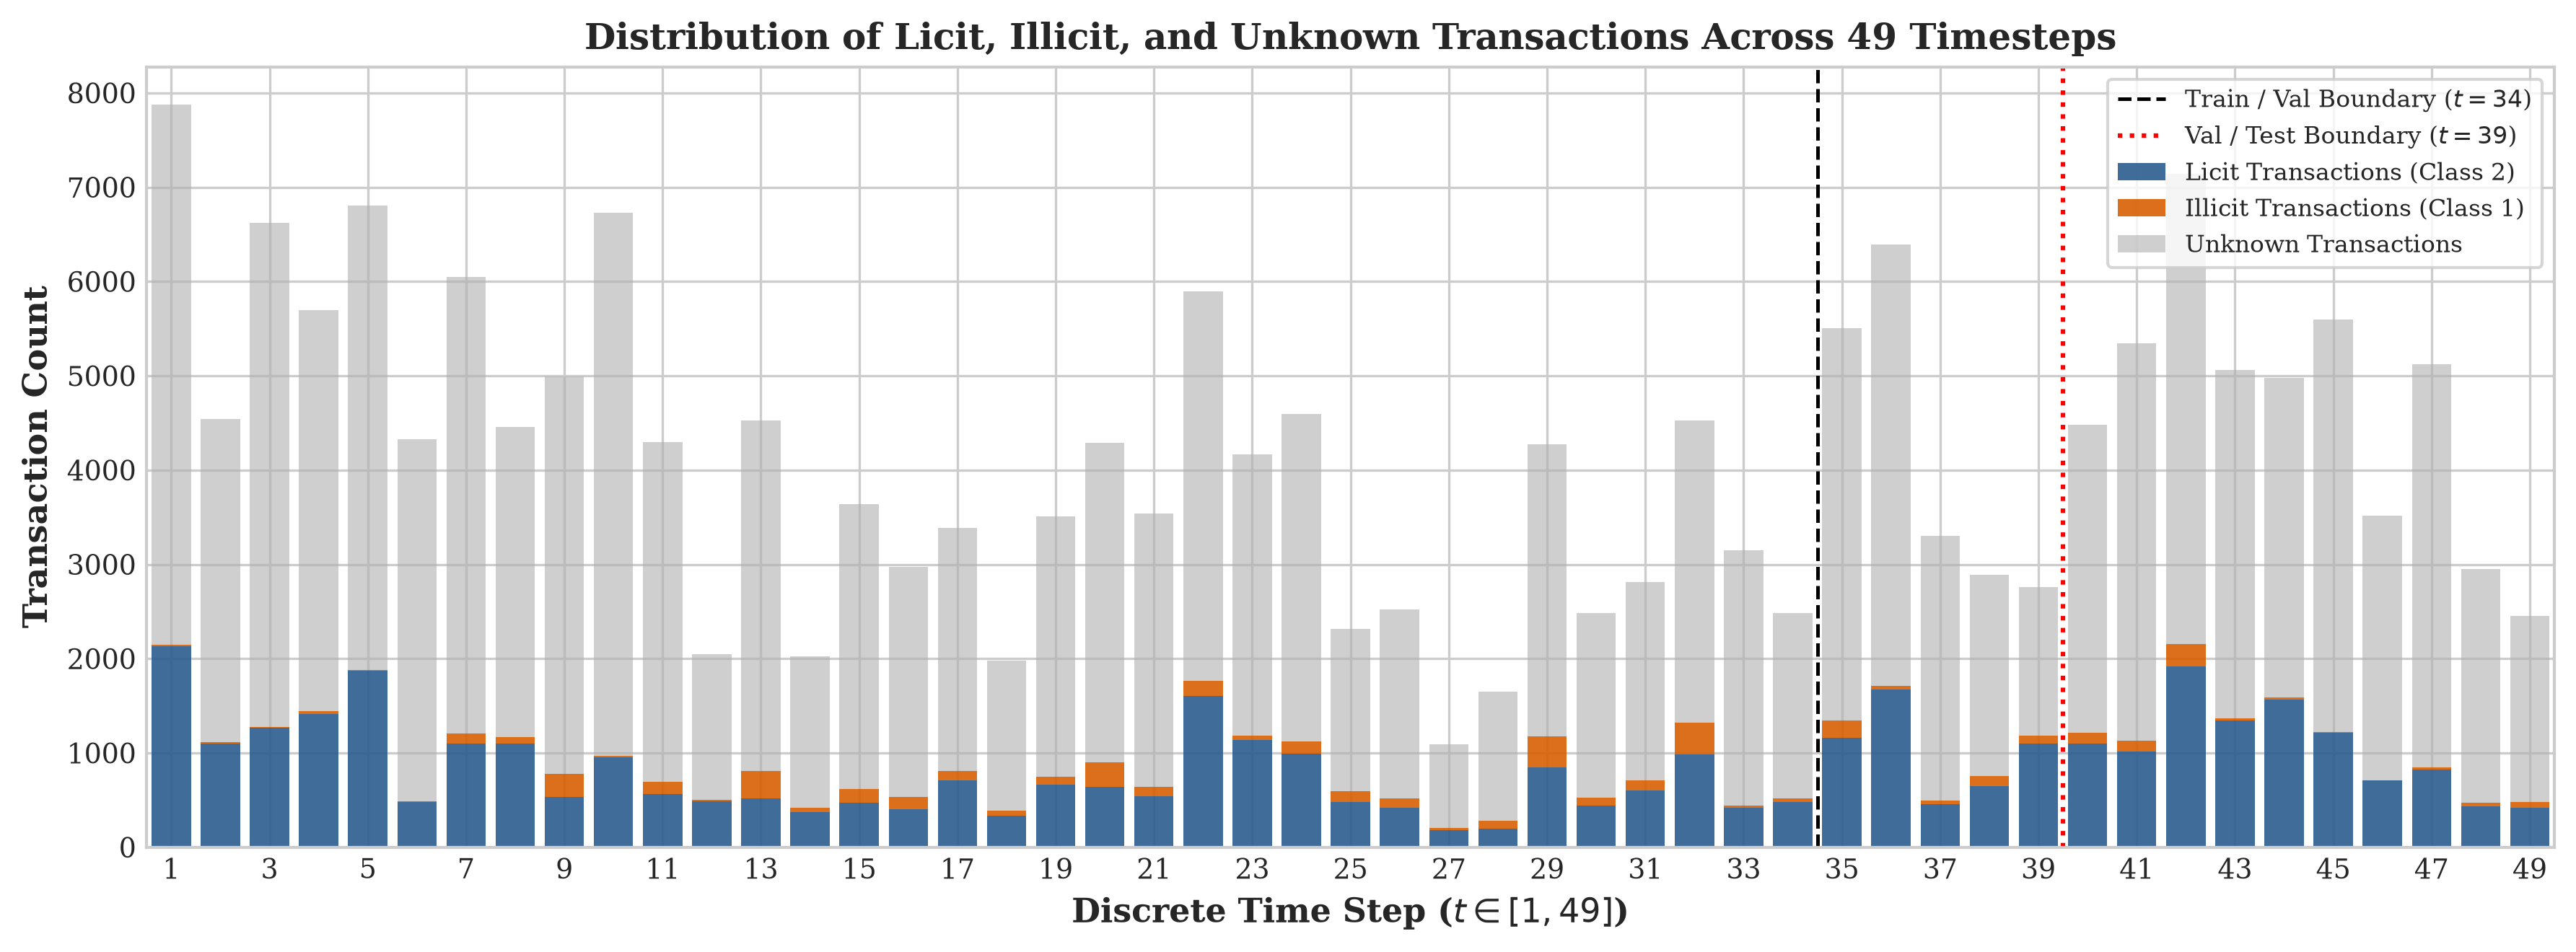
\includegraphics[width=\columnwidth]{../figures/label_distribution.png}
\caption{Distribution of Licit, Illicit, and Unknown transactions across the 49 discrete timesteps in the Elliptic benchmark dataset.}
\label{fig:label_distribution}
\end{figure}

\subsection{Evaluation Metrics under Class Skew}
Given severe class imbalance, overall accuracy is uninformative \cite{davis2006relationship, saito2015precision}. We evaluate minority-class detection using:
\begin{equation}
\text{Precision (P)} = \frac{\text{TP}}{\text{TP} + \text{FP}}
\label{eq:prec}
\end{equation}
\begin{equation}
\text{Recall (R)} = \frac{\text{TP}}{\text{TP} + \text{FN}}
\label{eq:rec}
\end{equation}
\begin{equation}
\text{F1-Score} = \frac{2 \cdot \text{P} \cdot \text{R}}{\text{P} + \text{R}}
\label{eq:f1}
\end{equation}
\begin{equation}
\text{MCC} = \frac{\text{TP} \cdot \text{TN} - \text{FP} \cdot \text{FN}}{\sqrt{(\text{TP}+\text{FP})(\text{TP}+\text{FN})(\text{TN}+\text{FP})(\text{TN}+\text{FN})}}
\label{eq:mcc}
\end{equation}
Our primary target metric is the \textbf{Illicit-Class F1-Score} on the blind test holdout ($t \in [40, 49]$), supported by \textbf{Precision-Recall Area Under the Curve (PR-AUC)}.

\subsection{Feature Space Representation}
Each transaction node $v \in V$ possesses a $165$-dimensional feature vector $x_v \in \mathbb{R}^{165}$ consisting of:
\begin{enumerate}
    \item \textbf{Local Features ($1$--$93$, $d_{\text{local}} = 93$):} Intrinsic metadata, including transaction fees, transacted volumes, input/output counts, and script properties.
    \item \textbf{Aggregated Features ($94$--$165$, $d_{\text{agg}} = 72$):} Handcrafted 1-hop summary statistics (minimum, maximum, mean, standard deviation) computed across immediate predecessor and successor transactions \cite{weber2019elliptic}.
\end{enumerate}

\subsection{Chronological Partitioning Protocol}
To evaluate prospective temporal generalization, we enforce a strict chronological split (see Fig. 2 and Table I):
\begin{itemize}
    \item \textbf{Training Set ($t \in [1, 34]$):} $29,894$ labeled nodes ($3,462$ illicit, $26,432$ licit; $11.58\%$ illicit prevalence).
    \item \textbf{Validation Set ($t \in [35, 39]$):} $5,486$ labeled nodes ($447$ illicit, $5,039$ licit; $8.15\%$ illicit prevalence).
    \item \textbf{Test Set ($t \in [40, 49]$):} $11,184$ labeled nodes ($636$ illicit, $10,548$ licit; $5.69\%$ illicit prevalence).
\end{itemize}

\begin{figure}[htbp]
\centering
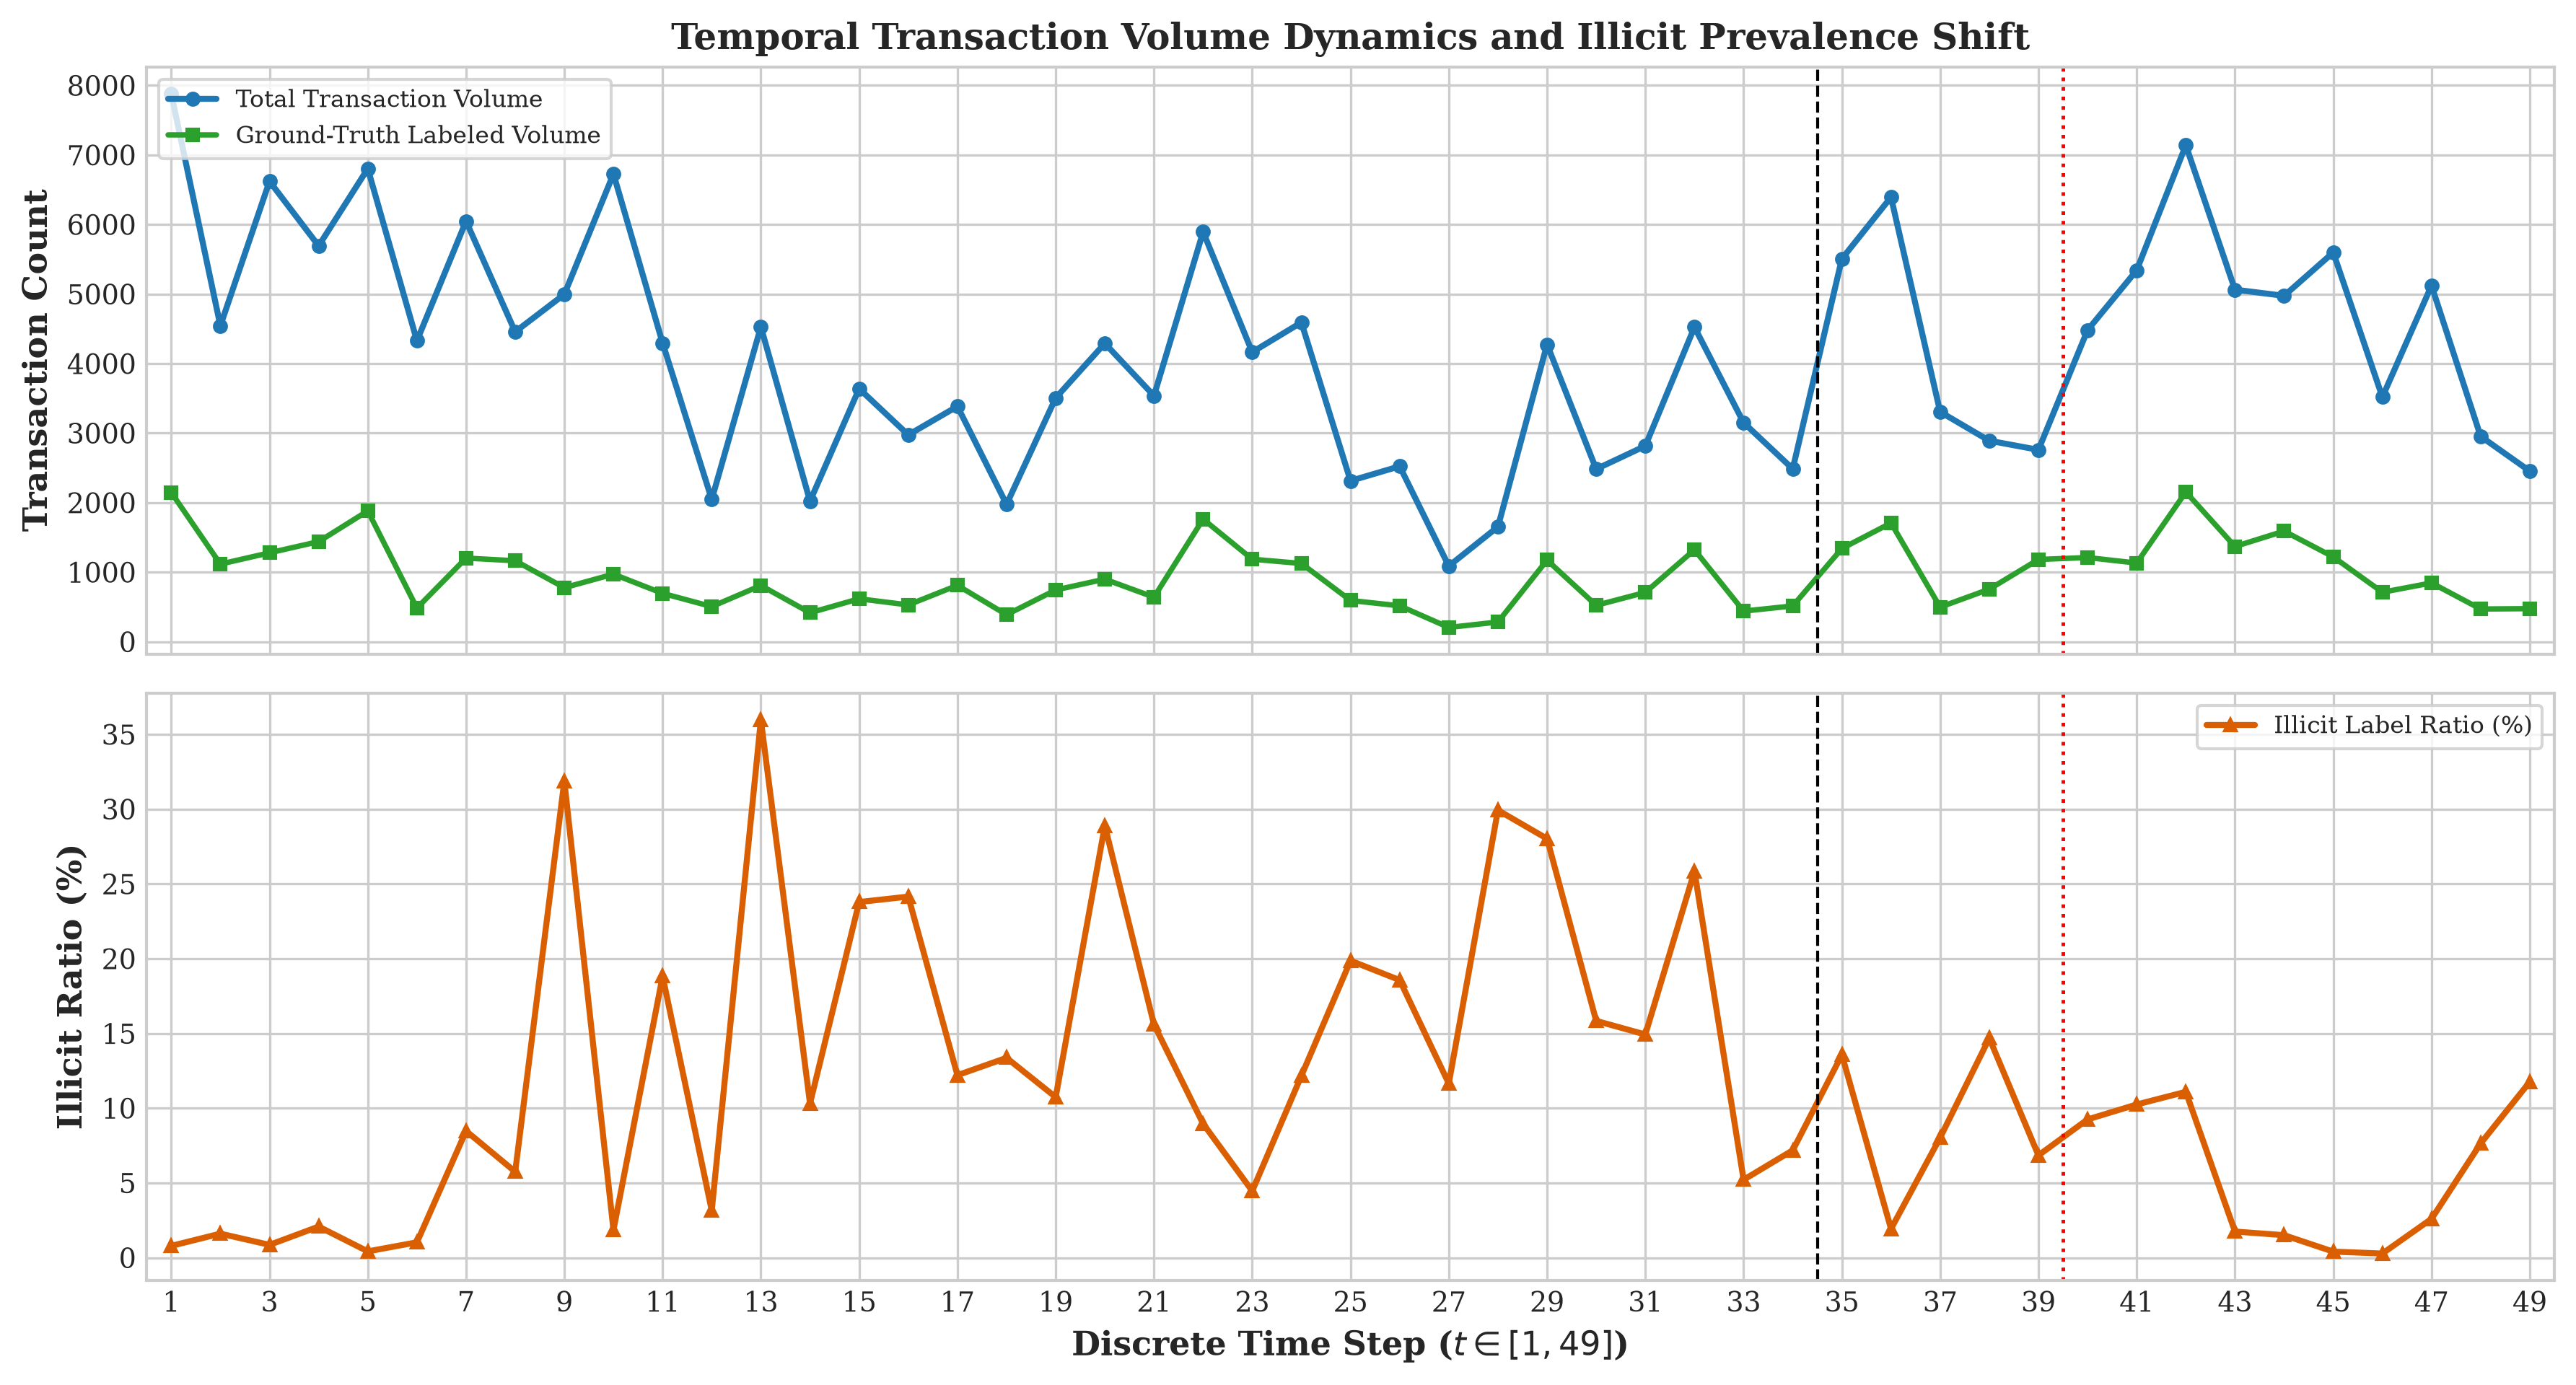
\includegraphics[width=\columnwidth]{../figures/temporal_evolution.png}
\caption{Total transaction volume and temporal class composition over the 49 discrete timesteps, showing chronological training, validation, and test partitions.}
\label{fig:temporal_evolution}
\end{figure}

\begin{table*}[t]
\centering
\caption{Elliptic Dataset Structure and Temporal Split Summary}
\label{tab:dataset_splits}
\begin{tabular}{lcccc}
\toprule
\textbf{Metric / Attribute} & \textbf{Training Partition} & \textbf{Validation Partition} & \textbf{Test Partition} & \textbf{Full Dataset} \\
\midrule
Timestep Range ($t$) & Timesteps 1--34 & Timesteps 35--39 & Timesteps 40--49 & Timesteps 1--49 \\
Discrete Time Steps & 34 snapshots & 5 snapshots & 10 snapshots & 49 snapshots \\
Labeled Transactions & 29,894 (64.18\%) & 5,486 (11.78\%) & 11,184 (24.04\%) & 46,564 (100.0\%) \\
Licit Transactions & 26,432 (88.42\%) & 5,039 (91.85\%) & 10,548 (94.31\%) & 42,019 (90.24\%) \\
Illicit Transactions & 3,462 (11.58\%) & 447 (8.15\%) & 636 (5.69\%) & 4,545 (9.76\%) \\
Imbalance Ratio (Licit : Illicit) & 7.63 : 1 & 11.27 : 1 & 16.58 : 1 & 9.245 : 1 \\
Total Graph Nodes (incl. Unknown) & 136,005 & 23,790 & 43,974 & 203,769 \\
Total Graph Edges & 156,589 & 27,243 & 50,523 & 234,355 \\
\bottomrule
\end{tabular}
\end{table*}

\section{Methodology}

\subsection{Baseline Model Architectures}
We benchmark against four conventional machine learning baselines:
\begin{itemize}
    \item \textbf{Logistic Regression (LR):} Linear classification optimized via L-BFGS with $L_2$ regularization ($C = 1.0$).
    \item \textbf{Random Forest (RF):} Bagged ensemble of 100 decision trees (\texttt{n\_estimators=100}, \texttt{max\_depth=None}, \texttt{min\_samples\_split=2}) \cite{breiman2001random}.
    \item \textbf{XGBoost:} Gradient-boosted decision trees (\texttt{n\_estimators=100}, \texttt{max\_depth=6}, \texttt{learning\_rate=0.1}, \texttt{subsample=0.8}, \texttt{colsample\_bytree=0.8}) \cite{chen2016xgboost}.
    \item \textbf{Multi-Layer Perceptron (MLP):} Deep neural network with 2 hidden layers (128 units each), ReLU activations, Dropout ($p=0.3$), Batch Normalization, trained via Adam ($lr=0.001$, weight decay $10^{-5}$).
\end{itemize}

\subsection{Graph Neural Network Architectures}
We evaluate three foundational Graph Neural Network architectures:
\begin{itemize}
    \item \textbf{Graph Convolutional Networks (GCN) \cite{kipf2017semi}:}
    \begin{equation}
    H^{(l+1)} = \sigma\left( \tilde{D}^{-\frac{1}{2}} \tilde{A} \tilde{D}^{-\frac{1}{2}} H^{(l)} W^{(l)} \right)
    \label{eq:gcn}
    \end{equation}
    \item \textbf{GraphSAGE \cite{hamilton2017inductive}:}
    \begin{equation}
    h_v^{(l+1)} = \sigma\left( W^{(l)} \cdot \left[ h_v^{(l)} \,\|\, \frac{1}{|\mathcal{N}(v)|} \sum_{u \in \mathcal{N}(v)} h_u^{(l)} \right] \right)
    \label{eq:sage}
    \end{equation}
    \item \textbf{Graph Attention Networks (GAT) \cite{velickovic2018graph}:}
    \begin{equation}
    \alpha_{vu} = \frac{\exp\left(\text{LeakyReLU}\left(a^T [W h_v \,\|\, W h_u]\right)\right)}{\sum_{k \in \mathcal{N}(v)} \exp\left(\text{LeakyReLU}\left(a^T [W h_v \,\|\, W h_k]\right)\right)}
    \label{eq:gat}
    \end{equation}
\end{itemize}
All GNN models employ 2 message-passing layers, 128 hidden channels, Dropout ($p=0.3$), and Adam optimizer ($lr=0.001$). GAT utilizes 4 attention heads (32 channels per head). Hyperparameter details are provided in Table II.

\begin{table}[htbp]
\centering
\caption{Model Architecture and Hyperparameter Specification}
\label{tab:model_spec}
{\small
\resizebox{\columnwidth}{!}{
\begin{tabular}{llp{3.8cm}}
\toprule
\textbf{Model} & \textbf{Family} & \textbf{Key Hyperparameters} \\
\midrule
Logistic Reg. & Linear & $C=1.0$, $L_2$ penalty, L-BFGS solver \\
Random Forest & Bagged Trees & 100 trees, unlimited depth, Gini split \\
XGBoost & Boosting & 100 trees, depth 6, lr 0.1, sub 0.8 \\
MLP & Neural Net & 2 layers, 128 units, Dropout 0.3, Adam \\
GCN & Graph Conv & 2 layers, 128 hidden, Adam ($10^{-3}$) \\
GraphSAGE & Inductive GNN & 2 layers, 128 hidden, Mean aggregate \\
GAT & Attention GNN & 2 layers, 128 hidden, 4 heads (32/head) \\
\bottomrule
\end{tabular}
}
}
\end{table}

\subsection{Loss Formulations and Cost-Sensitive Weighting}
We evaluate unweighted cross-entropy alongside cost-sensitive class weighting ($w_{\text{pos}} = 26,432 / 3,462 \approx 7.6349$). Unknown-label nodes are retained in the graph for message passing but strictly masked out from supervised loss computation:
\begin{equation}
\mathcal{L}_{\text{masked}} = -\frac{1}{|\mathcal{V}_{\text{train}}^{\text{labeled}}|} \sum_{v \in \mathcal{V}_{\text{train}}^{\text{labeled}}} \left[ w_{\text{pos}} y_v \log \hat{y}_v + (1 - y_v) \log (1 - \hat{y}_v) \right]
\label{eq:loss}
\end{equation}

\subsection{Training and Threshold Locking Protocol}
Models are trained for 100 epochs on Timesteps 1--34 with Early Stopping (patience = 15) monitoring validation illicit F1 on Timesteps 35--39. Decision thresholds are tuned strictly on the validation partition ($\tau^* = \arg\max \text{F1}_{\text{val}}$) and locked prior to blind evaluation on Timesteps 40--49.

\subsection{Statistical Significance Testing Protocol}
All non-deterministic architectures are evaluated across $N = 5$ random seeds ($S = \{42, 123, 456, 789, 999\}$). Statistical comparisons between the validation-selected GNN and baselines employ two-sided paired $t$-tests with Holm-Bonferroni correction \cite{holm1979simple} and exact paired Wilcoxon signed-rank tests \cite{wilcoxon1945individual, demsar2006statistical}.

\section{Results}

\subsection{Main Comparison on Full Features}
Quantitative results on the full 165-feature representation across five seeds are reported in Table III and illustrated in Fig. 3:
\begin{itemize}
    \item \textbf{Random Forest (Standard):} Achieved test illicit F1 of $0.7247 \pm 0.0027$ and PR-AUC of $0.6599 \pm 0.0025$.
    \item \textbf{XGBoost (Standard):} Achieved test illicit F1 of $0.7131 \pm 0.0111$ and PR-AUC of $0.6744 \pm 0.0028$.
    \item \textbf{MLP (Standard):} Achieved test illicit F1 of $0.5848 \pm 0.0194$ and PR-AUC of $0.5115 \pm 0.0187$.
    \item \textbf{Logistic Regression (Standard):} Produced deterministic test illicit F1 of $0.4015$ and PR-AUC of $0.2754$.
    \item \textbf{GAT (Weighted):} Produced the highest full-feature GNN performance (F1 $0.3308 \pm 0.0602$, PR-AUC $0.2667 \pm 0.0695$).
    \item \textbf{GraphSAGE (Weighted):} Produced F1 of $0.2822 \pm 0.1248$ and PR-AUC of $0.2366 \pm 0.1386$.
    \item \textbf{GCN (Weighted):} Produced F1 of $0.2589 \pm 0.0639$ and PR-AUC of $0.2202 \pm 0.0703$.
\end{itemize}

\begin{table*}[t]
\centering
\caption{Main Benchmark Results on Full Features (165 Dimensions)}
\label{tab:main_results}
\begin{tabular}{llcccccc}
\toprule
\textbf{Model Architecture} & \textbf{Model Family} & \textbf{Feat.} & \textbf{Loss Form} & \textbf{Validation F1} & \textbf{Test Illicit F1} & \textbf{Test PR-AUC} & \textbf{Test Prec. / Rec.} \\
\midrule
Random Forest & Tree Ensemble & 165 & Standard & $0.9489 \pm 0.0023$ & $\mathbf{0.7247 \pm 0.0027}$ & $0.6599 \pm 0.0025$ & $0.9586 / 0.5827$ \\
XGBoost & Gradient Boosting & 165 & Standard & $0.9399 \pm 0.0053$ & $0.7131 \pm 0.0111$ & $\mathbf{0.6744 \pm 0.0028}$ & $0.9127 / 0.5855$ \\
MLP & Neural Network & 165 & Standard & $0.8212 \pm 0.0344$ & $0.5848 \pm 0.0194$ & $0.5115 \pm 0.0187$ & $0.7630 / 0.4761$ \\
Logistic Regression & Linear Model & 165 & Standard & $0.5921 \pm 0.0000$ & $0.4015 \pm 0.0000$ & $0.2754 \pm 0.0000$ & $0.3821 / 0.4230$ \\
GAT & Graph Attention & 165 & Weighted & $0.6006 \pm 0.0982$ & $0.3308 \pm 0.0602$ & $0.2667 \pm 0.0695$ & $0.2680 / 0.4412$ \\
GraphSAGE & Inductive GNN & 165 & Weighted & $0.4473 \pm 0.1590$ & $0.2822 \pm 0.1248$ & $0.2366 \pm 0.1386$ & $0.2695 / 0.3588$ \\
GCN & Graph Conv Net & 165 & Weighted & $0.4293 \pm 0.0923$ & $0.2589 \pm 0.0639$ & $0.2202 \pm 0.0703$ & $0.2788 / 0.2884$ \\
\bottomrule
\end{tabular}
\end{table*}

\begin{figure}[htbp]
\centering
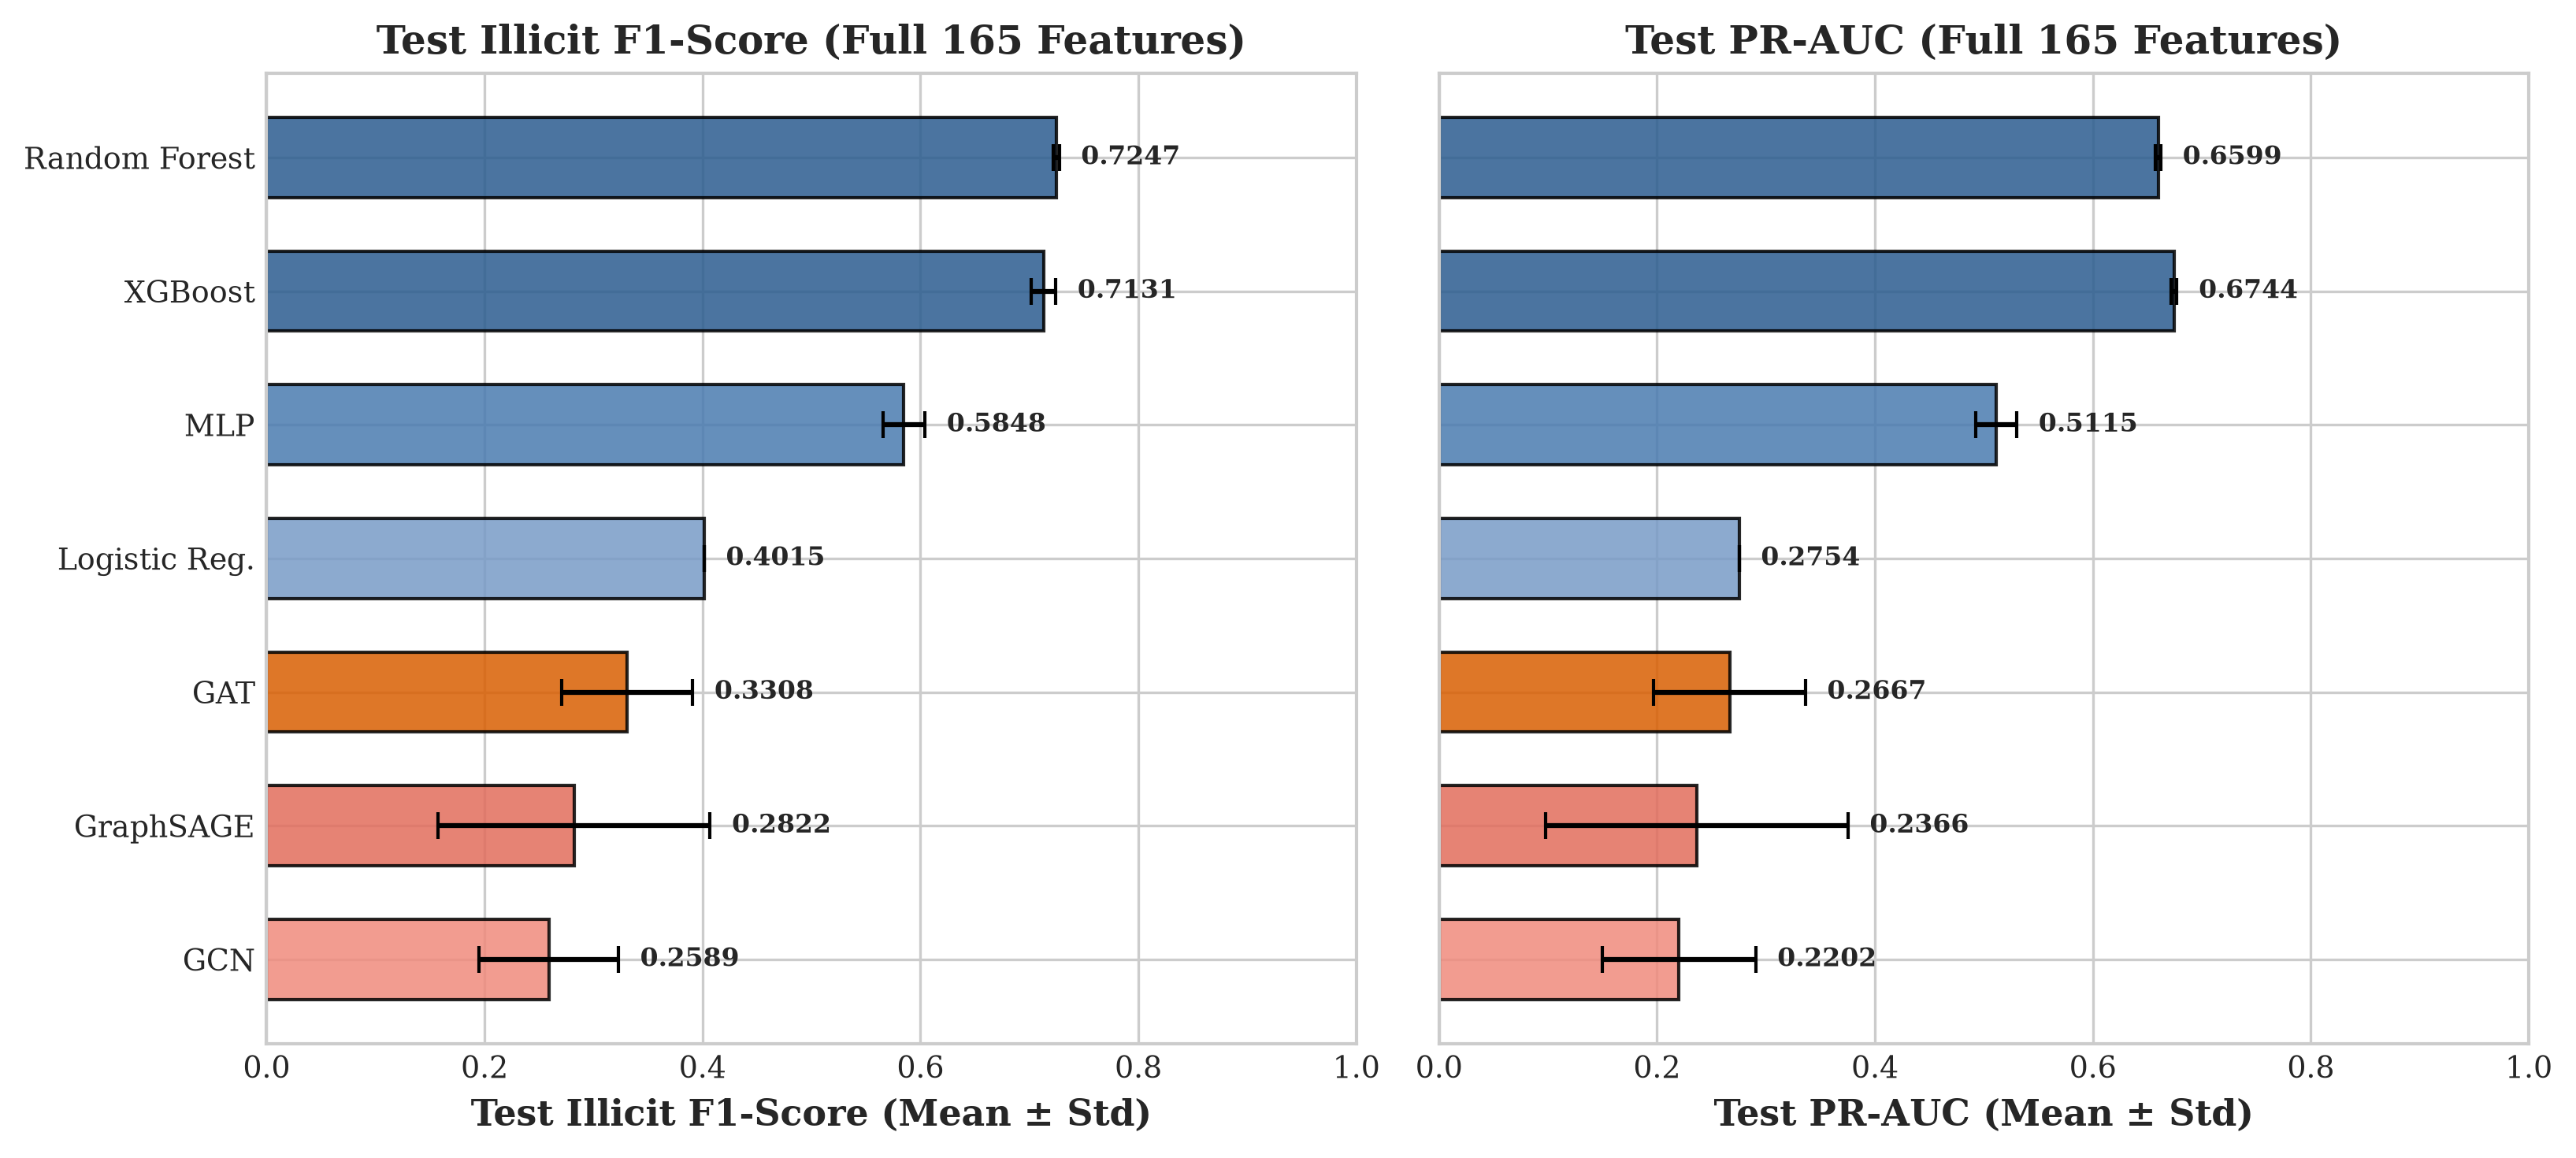
\includegraphics[width=\columnwidth]{../figures/gnn_vs_conventional_baselines.png}
\caption{Main benchmark comparison of test illicit F1-score and PR-AUC between conventional tabular machine learning baselines and Graph Neural Network architectures on the 165-feature representation.}
\label{fig:main_benchmark}
\end{figure}

\subsection{F1 and PR-AUC Dynamics}
For XGBoost, continuous ranking quality was superior (PR-AUC $0.6744$) despite Random Forest obtaining a marginally higher discrete F1 ($0.7247$ vs. $0.7131$). Across GNNs, test F1 and PR-AUC tracked closely together ($0.3308$ vs. $0.2667$ for GAT; $0.2822$ vs. $0.2366$ for GraphSAGE; $0.2589$ vs. $0.2202$ for GCN).

\subsection{Precision-Recall Trade-offs}
Precision-Recall dynamics (see Fig. 4) reveal that tree ensembles achieved exceptionally high precision ($0.9586$ for RF; $0.9127$ for XGBoost) at moderate recall ($\approx 0.58$), whereas GNN architectures produced lower precision ($0.2680$--$0.2788$) and moderate recall ($0.2884$--$0.4412$).

\begin{figure}[htbp]
\centering
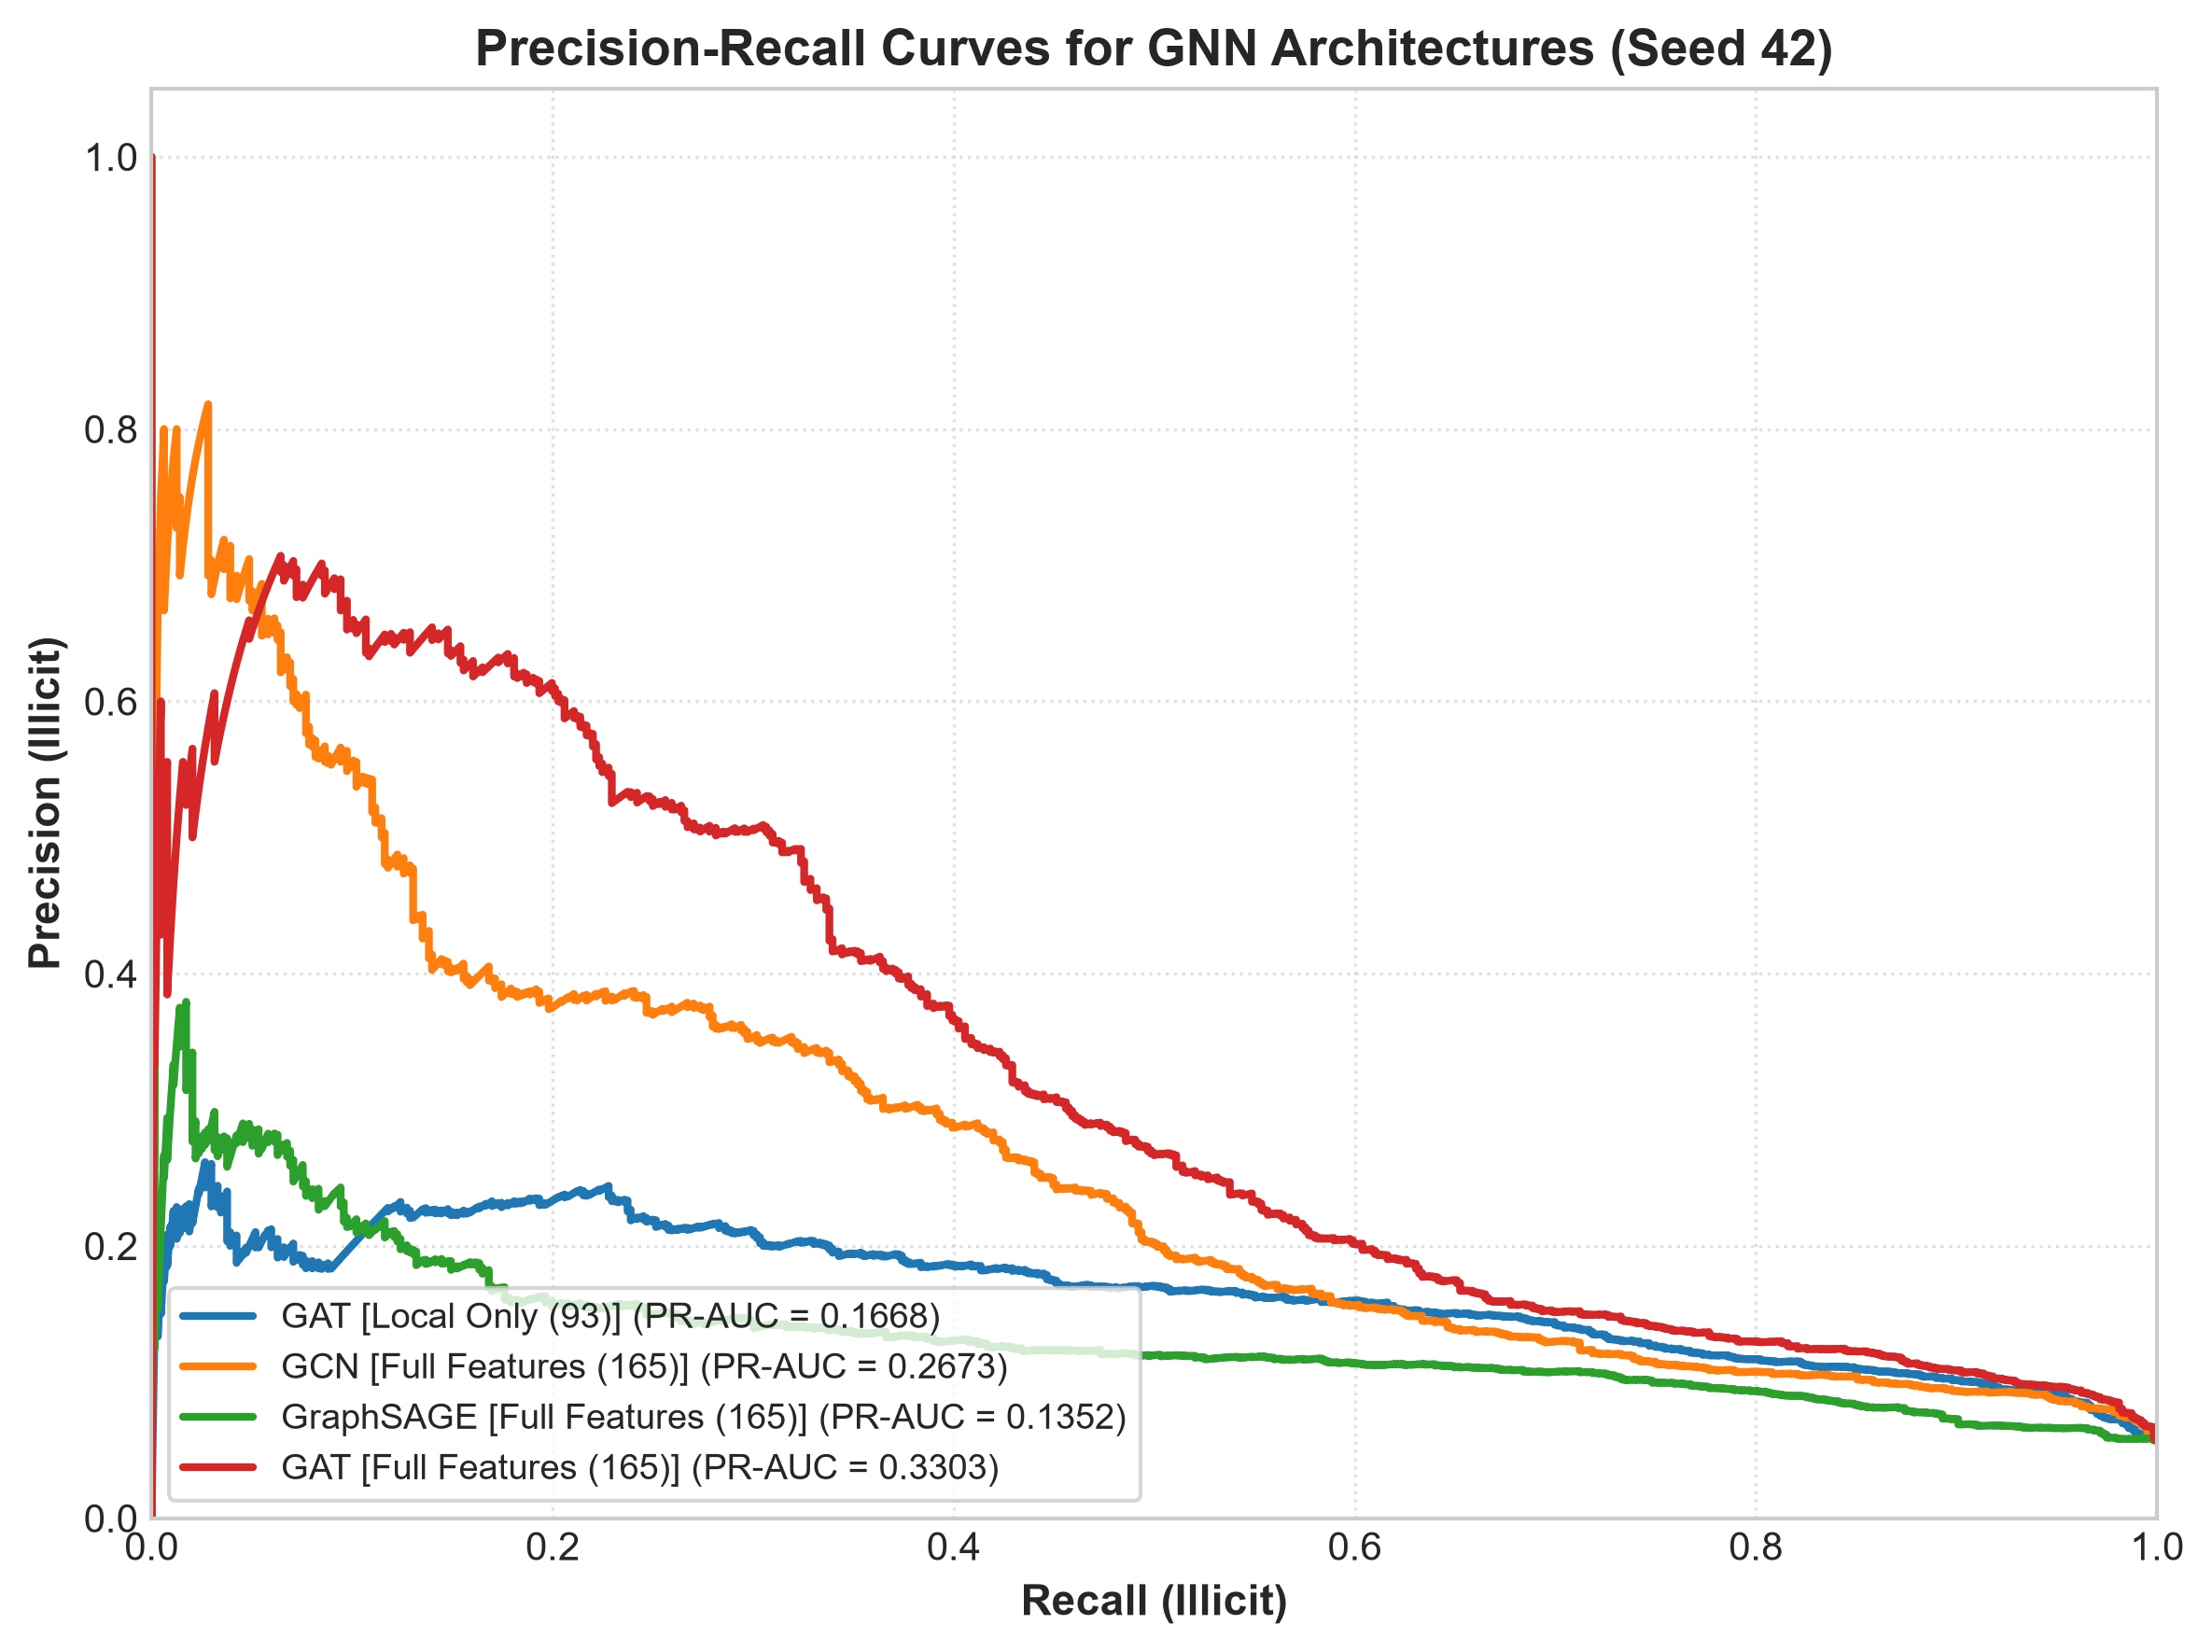
\includegraphics[width=\columnwidth]{../figures/gnn_precision_recall_curves.png}
\caption{Precision-Recall curves for primary Graph Neural Network architectures evaluated on the blind test holdout partition across timesteps 40–49.}
\label{fig:pr_curves}
\end{figure}

\subsection{Local versus Full Feature Representations}
Table IV and Fig. 5 compare models trained on Local 93 features versus Full 165 features:
\begin{itemize}
    \item Tree ensembles and MLP benefited consistently from 1-hop aggregate features (RF: $+0.0311$; XGB: $+0.0430$; MLP: $+0.0187$).
    \item GAT test F1 improved by $+0.0942$ ($0.2367 \to 0.3308$).
    \item In contrast, GraphSAGE achieved its highest performance on 93 Local features ($0.4153 \pm 0.1914$), declining by $-0.1331$ on Full features ($0.2822 \pm 0.1248$).
    \item GCN was largely invariant ($\Delta\text{F1} = +0.0030$).
\end{itemize}

\begin{table}[htbp]
\centering
\caption{Feature Representation Comparison (Local 93 vs. Full 165)}
\label{tab:feat_comp}
{\small
\resizebox{\columnwidth}{!}{
\begin{tabular}{lcccc}
\toprule
\textbf{Model} & \textbf{Local 93 F1} & \textbf{Full 165 F1} & \textbf{$\Delta$F1} & \textbf{$\Delta$PR-AUC} \\
\midrule
Random Forest & $0.6936 \pm 0.0022$ & $\mathbf{0.7247 \pm 0.0027}$ & $+0.0311$ & $+0.0267$ \\
XGBoost & $0.6701 \pm 0.0069$ & $0.7131 \pm 0.0111$ & $+0.0430$ & $+0.0355$ \\
MLP & $0.5661 \pm 0.0232$ & $0.5848 \pm 0.0194$ & $+0.0187$ & $+0.0227$ \\
Logistic Reg. & $0.4378 \pm 0.0000$ & $0.4015 \pm 0.0000$ & $-0.0363$ & $-0.0252$ \\
GAT & $0.2367 \pm 0.0825$ & $0.3308 \pm 0.0602$ & $+0.0942$ & $+0.1014$ \\
GraphSAGE & $\mathbf{0.4153 \pm 0.1914}$ & $0.2822 \pm 0.1248$ & $-0.1331$ & $-0.1293$ \\
GCN & $0.2559 \pm 0.0768$ & $0.2589 \pm 0.0639$ & $+0.0030$ & $+0.0064$ \\
\bottomrule
\end{tabular}
}
}
\end{table}

\begin{figure}[htbp]
\centering
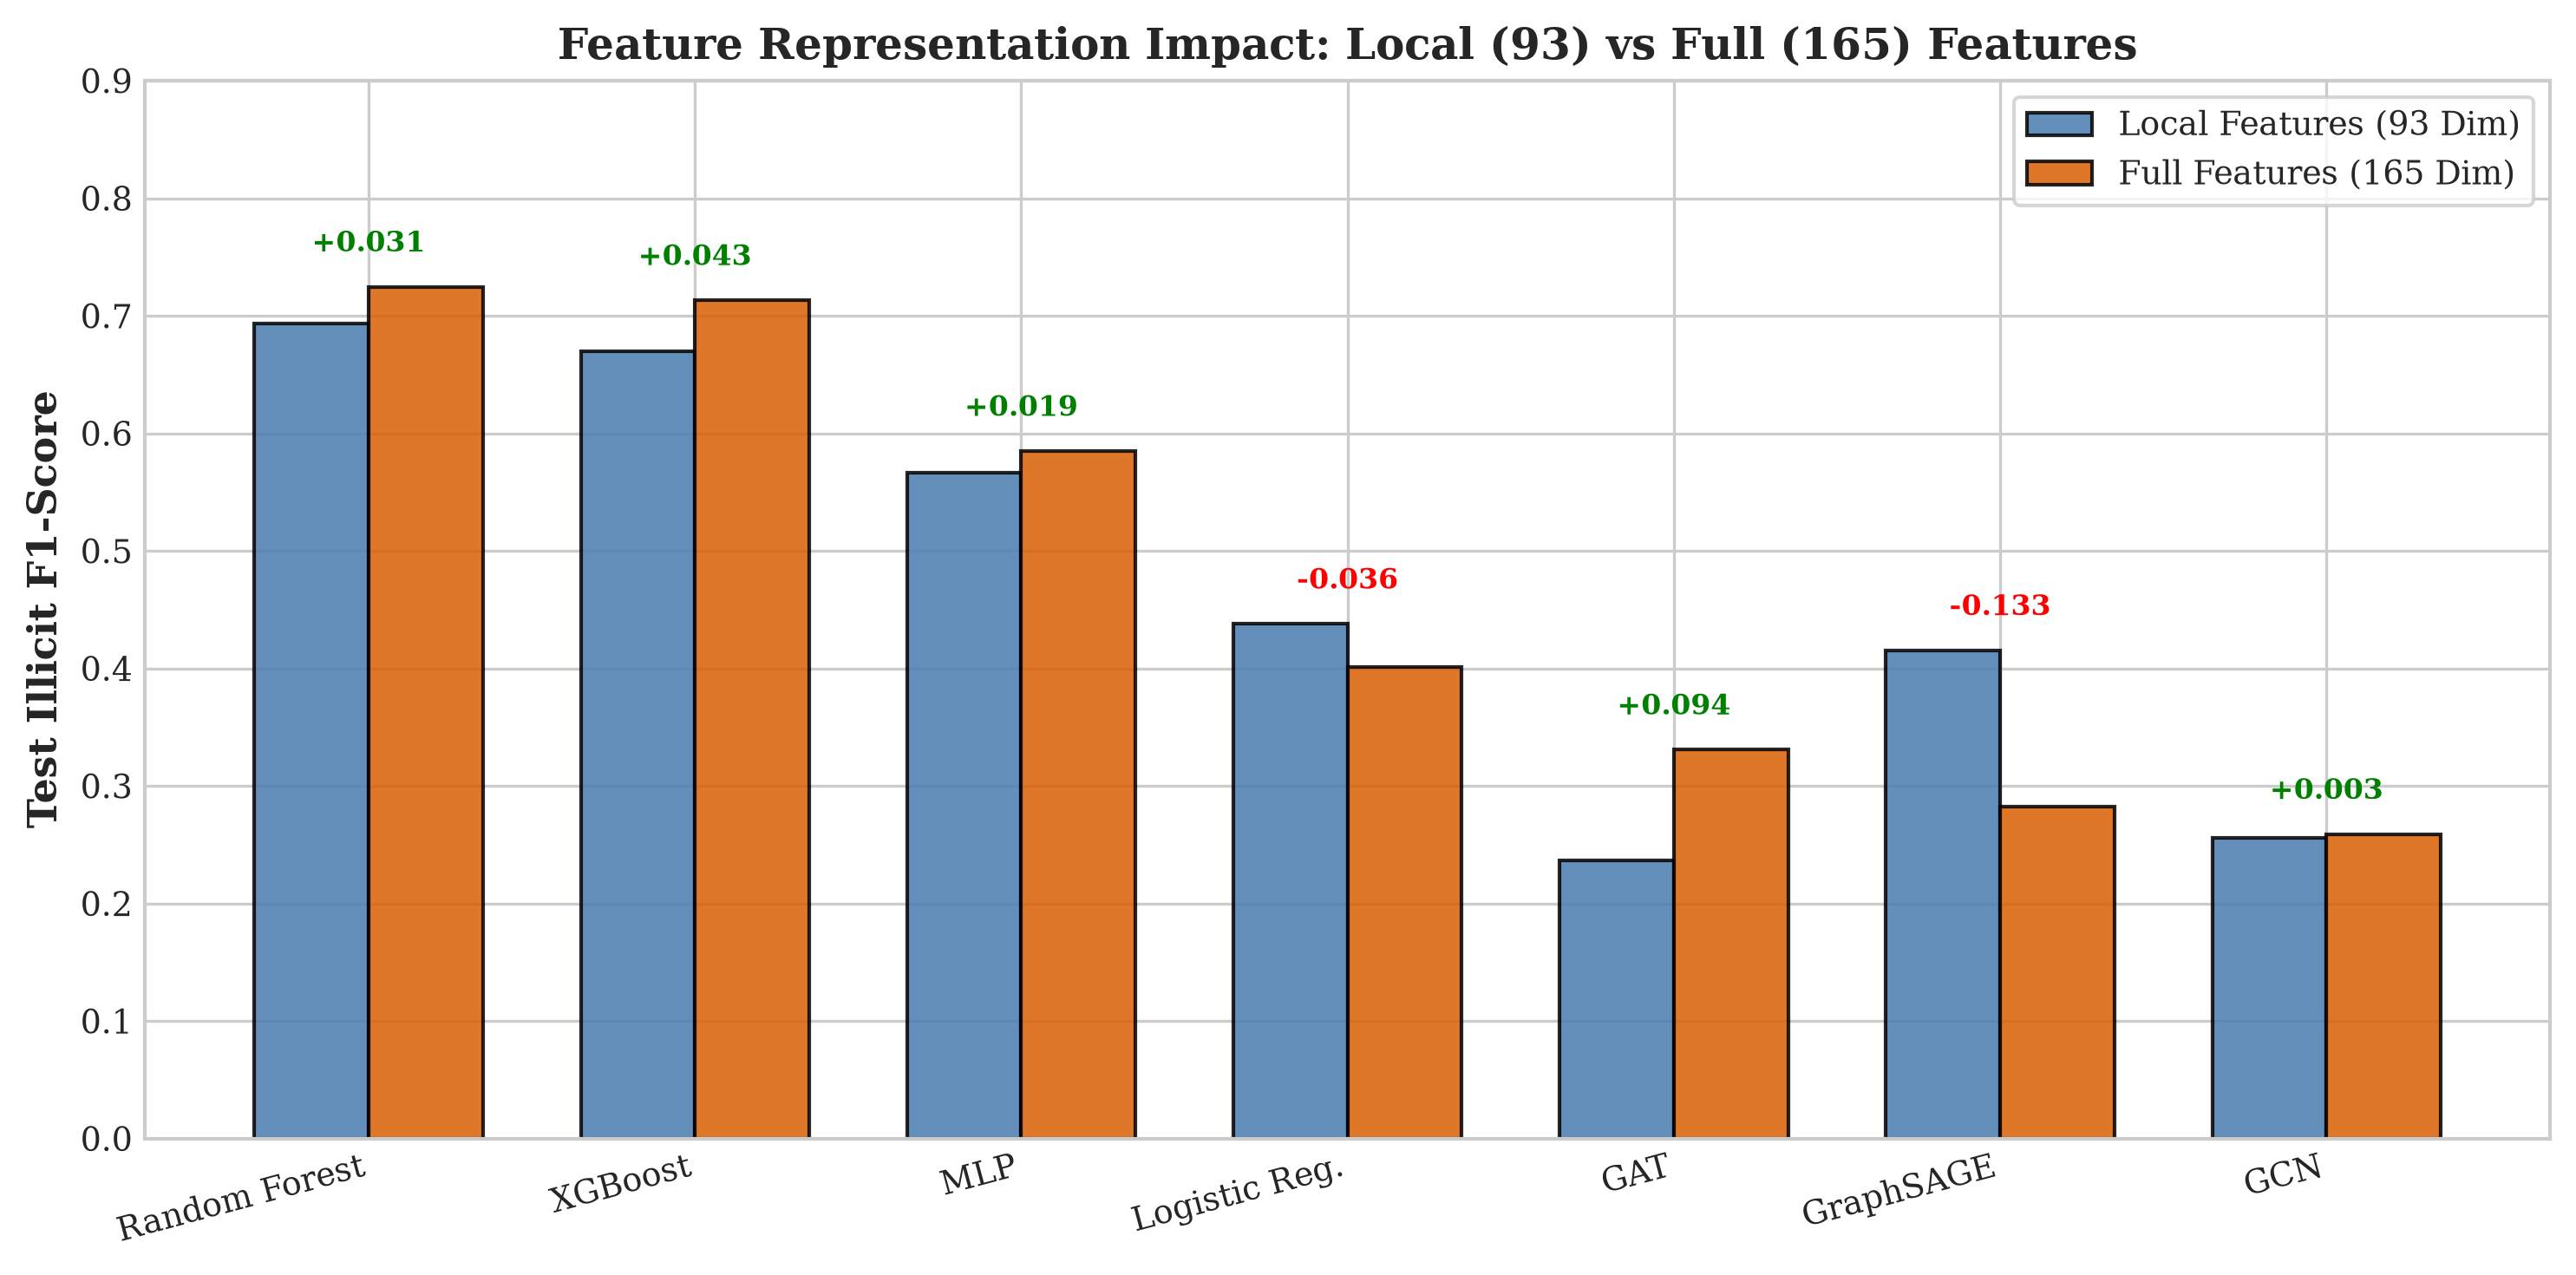
\includegraphics[width=\columnwidth]{../figures/feature_ablation_local_vs_full.png}
\caption{Feature representation impact comparing Local 93 metadata features against Full 165 features across conventional ML and GNN models.}
\label{fig:feat_ablation}
\end{figure}

\subsection{Standard versus Cost-Sensitive Loss Weighting}
As shown in Table V, positive-class loss weighting ($w_{\text{pos}} \approx 7.63$) shifted precision-recall operating points rather than providing universal F1 gains, as validation threshold tuning had already recalibrated unweighted models.

\begin{table}[htbp]
\centering
\caption{Class Loss Weighting Comparison (Full 165 Features)}
\label{tab:weight_comp}
{\small
\resizebox{\columnwidth}{!}{
\begin{tabular}{lcccc}
\toprule
\textbf{Model Architecture} & \textbf{Standard F1} & \textbf{Weighted F1} & \textbf{$\Delta$F1} & \textbf{MCC (Std)} \\
\midrule
Random Forest & $\mathbf{0.7247 \pm 0.0027}$ & $0.7024 \pm 0.0051$ & $-0.0223$ & $0.7367 \pm 0.0057$ \\
XGBoost & $0.7131 \pm 0.0111$ & $\mathbf{0.7197 \pm 0.0074}$ & $+0.0066$ & $0.7189 \pm 0.0154$ \\
MLP & $0.5848 \pm 0.0194$ & $0.5513 \pm 0.0362$ & $-0.0334$ & $0.5840 \pm 0.0155$ \\
Logistic Reg. & $0.4015 \pm 0.0000$ & $0.3480 \pm 0.0000$ & $-0.0535$ & $0.3640 \pm 0.0000$ \\
\bottomrule
\end{tabular}
}
}
\end{table}

\subsection{Validation-to-Test Generalization Decay}
All architectures suffered marked performance declines from validation (Timesteps 35--39) to blind test (Timesteps 40--49):
\begin{equation}
\Delta_{\text{rel}} = \frac{\text{Val F1} - \text{Test F1}}{\text{Val F1}} \times 100
\label{eq:drop}
\end{equation}
Relative drops: RF: $-23.6\%$; XGBoost: $-24.1\%$; MLP: $-28.8\%$; GraphSAGE (Local): $-31.5\%$; GCN: $-39.7\%$; GAT: $-44.9\%$.

\subsection{Random-Seed Stability and Initialization Variance}
Table VI and Fig. 9 demonstrate that tree ensembles exhibited tight cross-seed clustering ($\sigma \le 0.0111$), while GNNs displayed wide dispersion across seeds (GraphSAGE Local range $\Delta = 0.3669$, GCN Full range $\Delta = 0.4686$).

\begin{table}[htbp]
\centering
\caption{Multi-Seed Stability and Parameter Initialization Sensitivity}
\label{tab:seed_stability}
{\small
\resizebox{\columnwidth}{!}{
\begin{tabular}{lcccc}
\toprule
\textbf{Model Configuration} & \textbf{Min F1} & \textbf{Max F1} & \textbf{Range ($\Delta$)} & \textbf{Mean $\pm$ Std F1} \\
\midrule
Random Forest (165) & 0.7209 & 0.7271 & 0.0062 & $0.7247 \pm 0.0027$ \\
XGBoost (165) & 0.6984 & 0.7223 & 0.0239 & $0.7131 \pm 0.0111$ \\
MLP (165) & 0.5520 & 0.5989 & 0.0469 & $0.5848 \pm 0.0194$ \\
Logistic Reg. (165) & 0.4015 & 0.4015 & 0.0000 & $0.4015 \pm 0.0000$ \\
GAT (165) & 0.2241 & 0.3638 & 0.1397 & $0.3308 \pm 0.0602$ \\
GraphSAGE (165) & 0.1477 & 0.4746 & 0.3269 & $0.2822 \pm 0.1248$ \\
GCN (165) & 0.1723 & 0.6409 & 0.4686 & $0.2589 \pm 0.0639$ \\
GraphSAGE (Local 93) & 0.2583 & 0.6252 & 0.3669 & $0.4153 \pm 0.1914$ \\
\bottomrule
\end{tabular}
}
}
\end{table}

\begin{figure}[htbp]
\centering
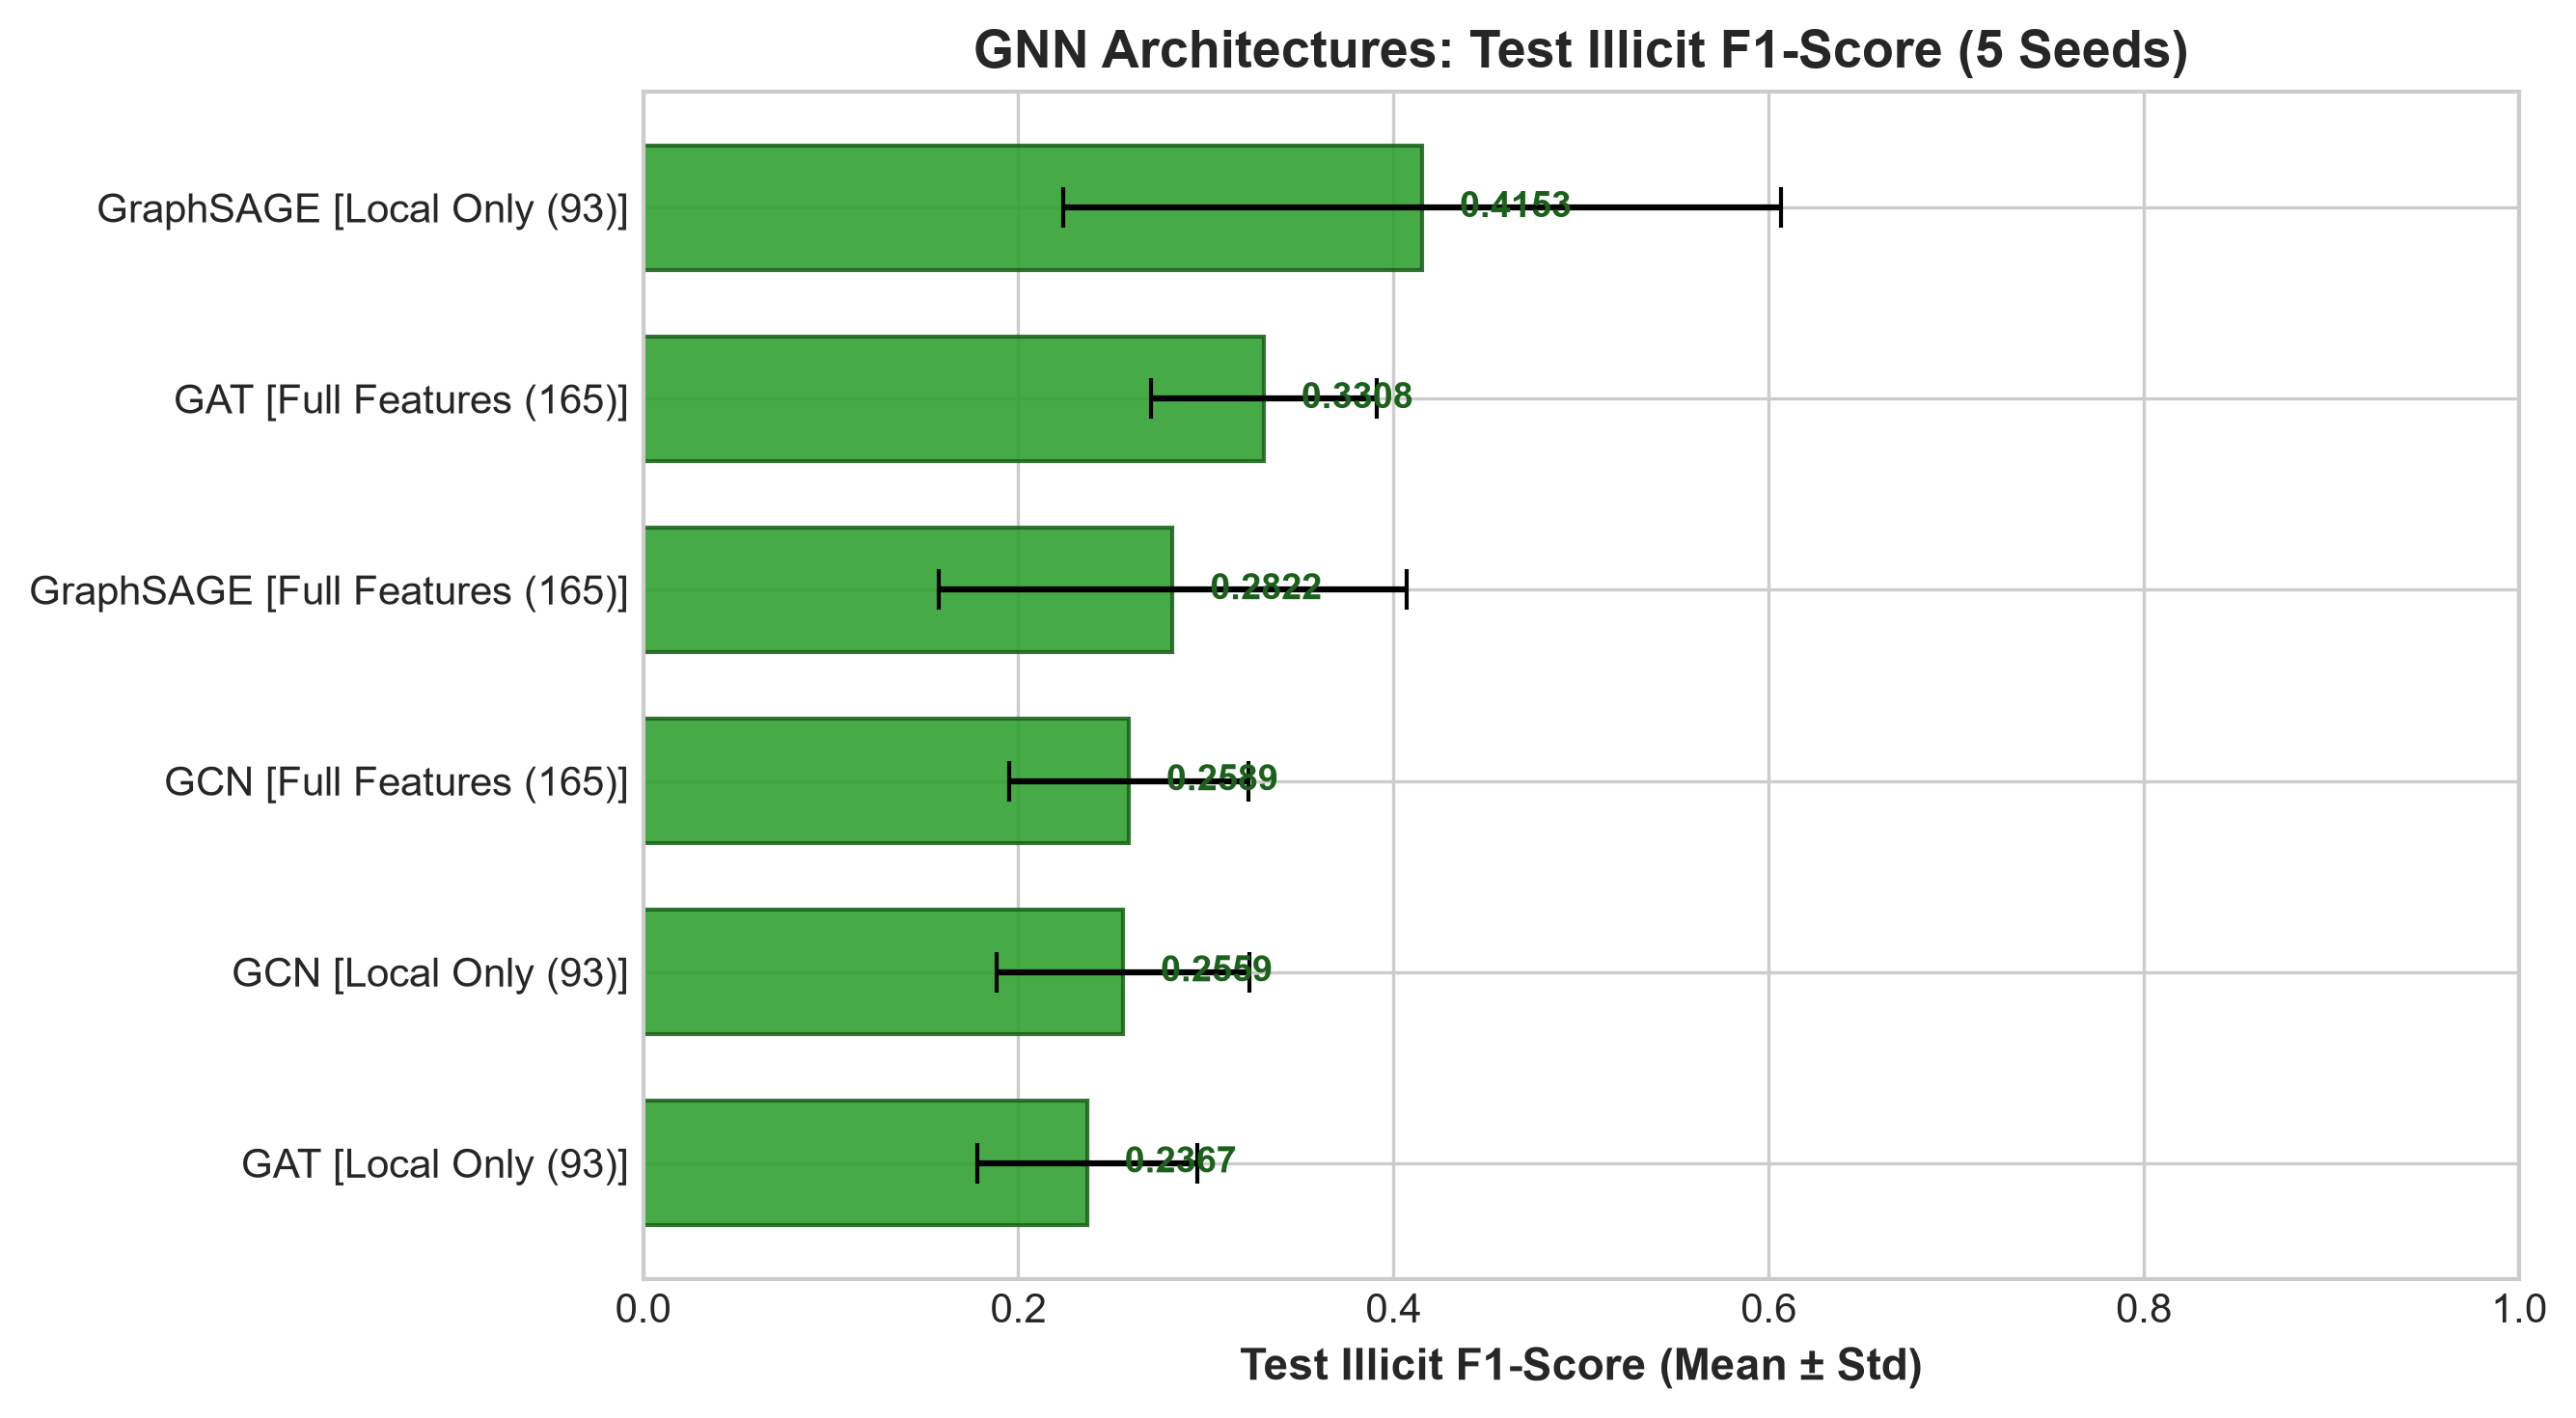
\includegraphics[width=\columnwidth]{../figures/gnn_model_comparison_f1.png}
\caption{Cross-seed test F1 score distributions and parameter initialization variance across five random seeds.}
\label{fig:seed_stability}
\end{figure}

\section{Ablation and Sensitivity Analysis}

\subsection{Impact of Unlabeled Graph Context}
Table VII and Fig. 6 present the ablation comparing the full $100\%$ topology against an induced subgraph of labeled nodes only:
\begin{itemize}
    \item For GCN, removing unknown nodes increased test illicit F1 from $0.2589$ to $0.4555$ ($\Delta = +0.1966$).
    \item For GraphSAGE, removing unknown nodes increased F1 from $0.2822$ to $0.4132$ ($\Delta = +0.1310$).
    \item For GAT, retaining unknown nodes produced higher F1 ($0.3308$ vs. $0.2918$).
\end{itemize}

\begin{table}[htbp]
\centering
\caption{Unknown-Node Context Ablation (Timesteps 40--49, 165 Features)}
\label{tab:unknown_ablation}
{\small
\resizebox{\columnwidth}{!}{
\begin{tabular}{lcccc}
\toprule
\textbf{Architecture} & \textbf{Retained F1} & \textbf{Removed F1} & \textbf{$\Delta$F1} & \textbf{Trend} \\
\midrule
GAT & $0.3308 \pm 0.0602$ & $0.2918 \pm 0.0521$ & $-0.0390$ & Retained Higher \\
GCN & $0.2589 \pm 0.0639$ & $0.4555 \pm 0.0524$ & $+0.1966$ & Removed Higher \\
GraphSAGE & $0.2822 \pm 0.1248$ & $0.4132 \pm 0.0514$ & $+0.1310$ & Removed Higher \\
\bottomrule
\end{tabular}
}
}
\end{table}

\begin{figure}[htbp]
\centering
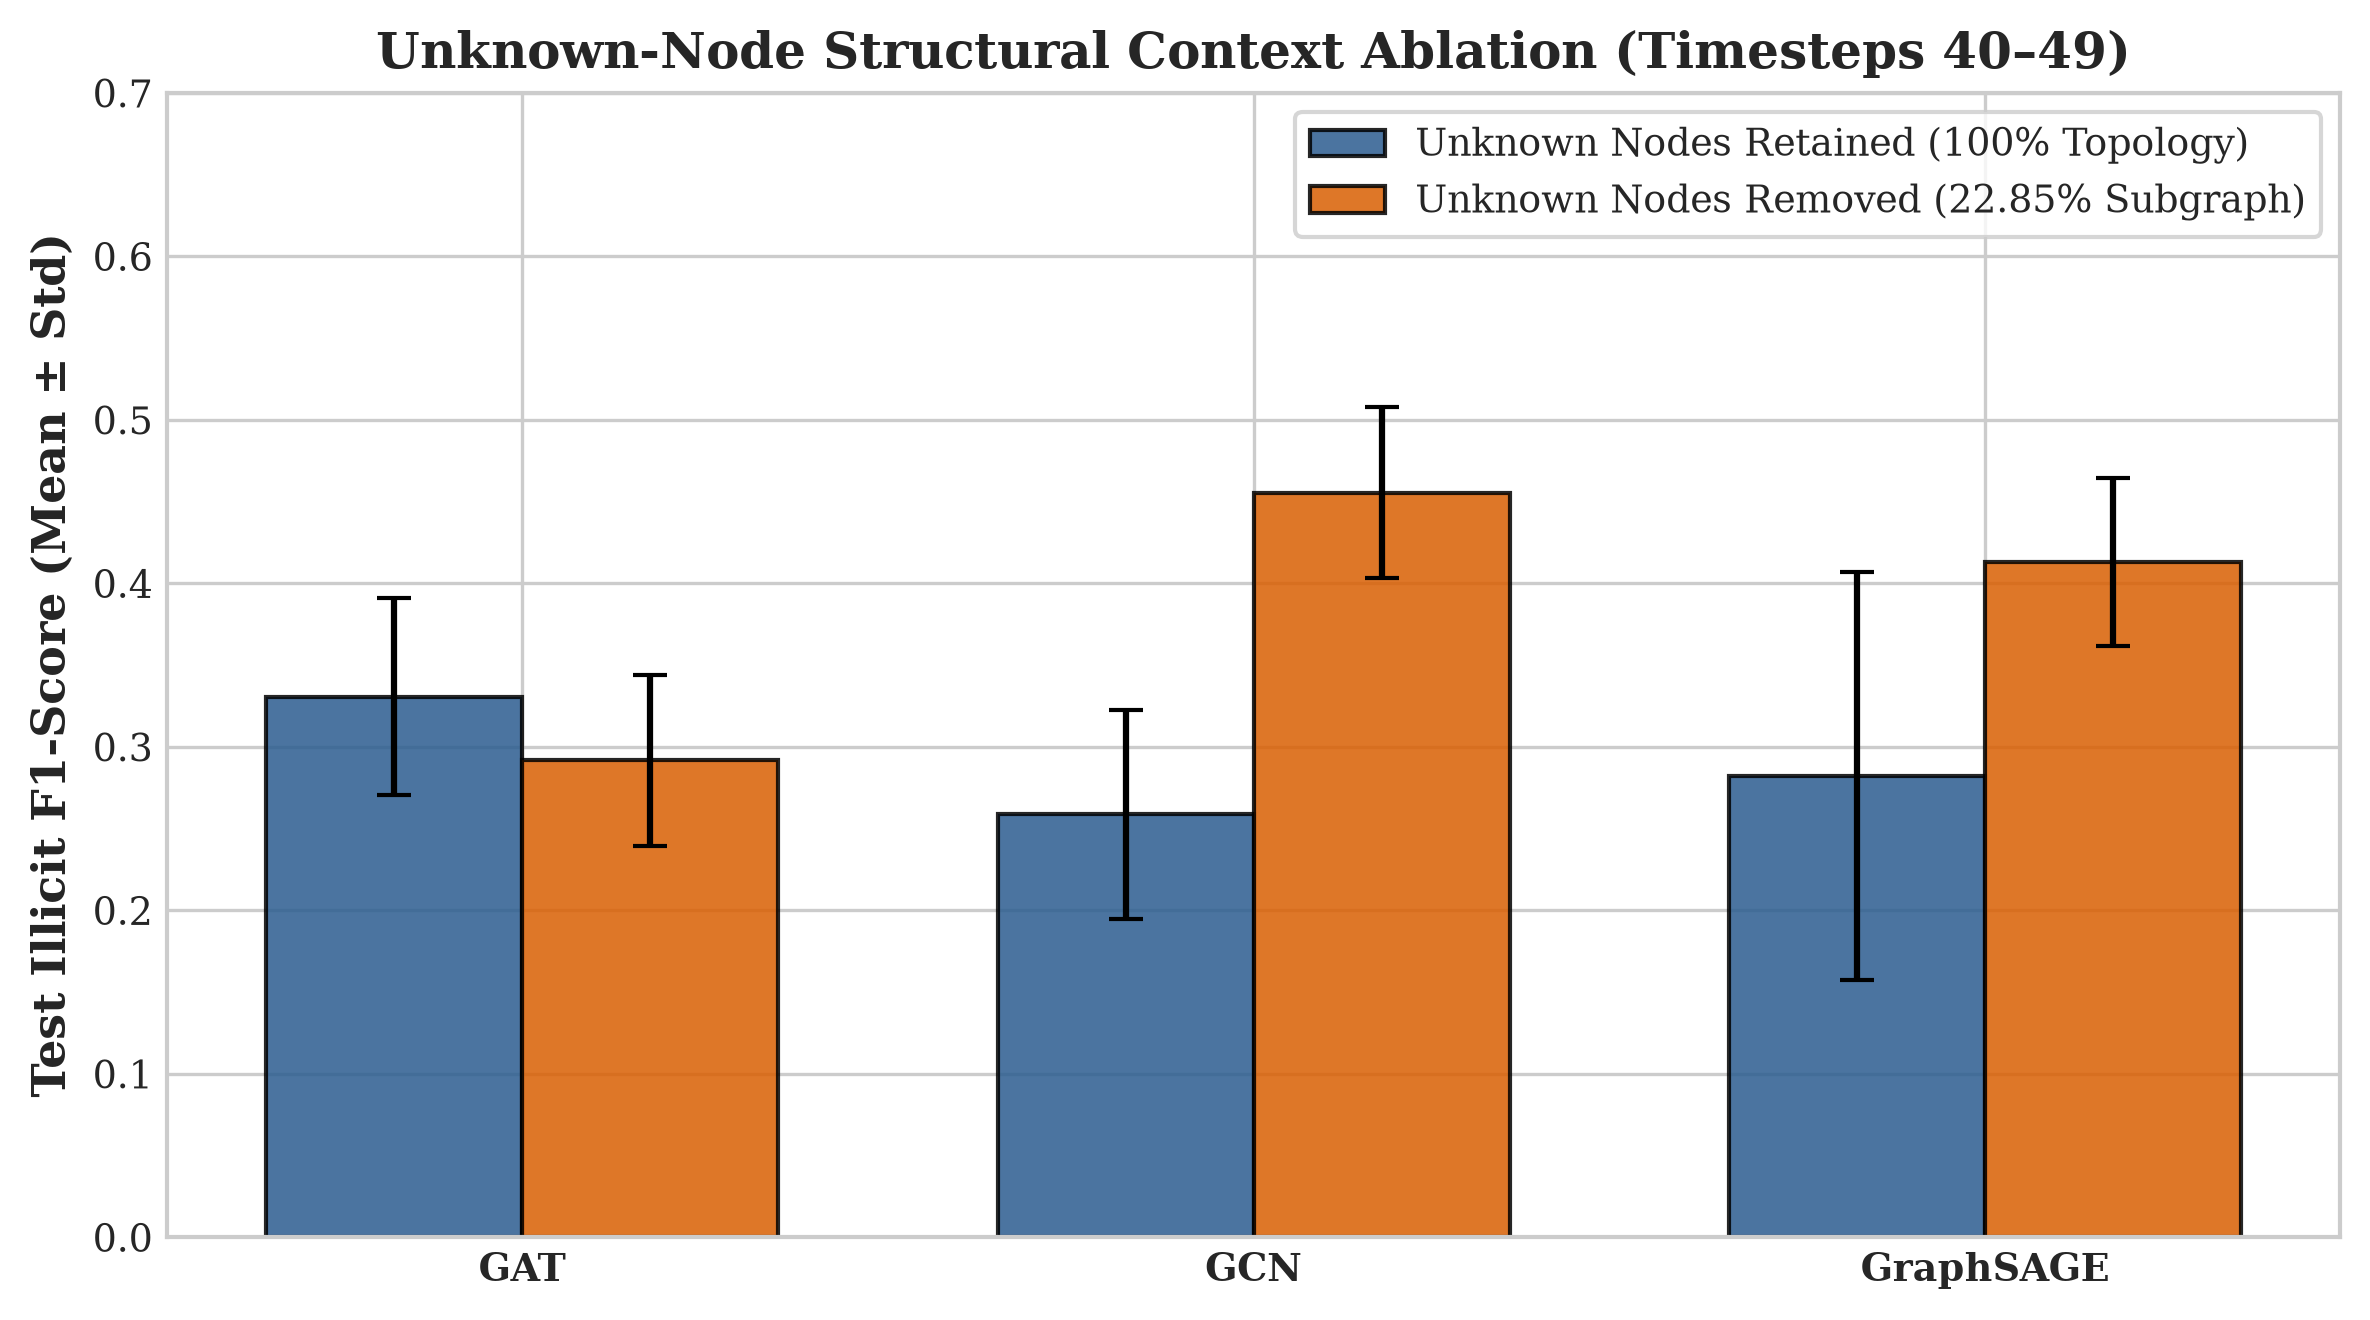
\includegraphics[width=\columnwidth]{../figures/unknown_node_ablation.png}
\caption{Unknown-node context ablation comparing test F1 performance when unlabeled transaction nodes are retained versus removed from the graph.}
\label{fig:unknown_ablation}
\end{figure}

\subsection{Graph Propagation Directionality}
Table VIII and Fig. 7 examine Forward ($u \to v$), Backward ($v \to u$), and Bidirectional message passing. Backward propagation yielded higher retrospective test F1 ($0.3213$--$0.3953$) than forward flow ($0.2589$--$0.3308$), and bidirectional propagation reached $0.4618$ for GAT. However, backward flow relies on future transactional context unavailable during live broadcast; forward flow remains the primary inductive standard.

\begin{table}[htbp]
\centering
\caption{Graph Directionality Ablation (Timesteps 40--49, 165 Features)}
\label{tab:direction_ablation}
{\small
\resizebox{\columnwidth}{!}{
\begin{tabular}{lcccc}
\toprule
\textbf{Architecture} & \textbf{Forward} & \textbf{Backward} & \textbf{Bidirectional} & \textbf{$\Delta$(Bwd-Fwd)} \\
\midrule
GAT & $0.3308 \pm 0.0602$ & $0.3938 \pm 0.0706$ & $0.4618 \pm 0.0234$ & $+0.0630$ \\
GCN & $0.2589 \pm 0.0639$ & $0.3953 \pm 0.0462$ & $0.3142 \pm 0.0571$ & $+0.1364$ \\
GraphSAGE & $0.2822 \pm 0.1248$ & $0.3213 \pm 0.0558$ & $0.3710 \pm 0.1228$ & $+0.0391$ \\
\bottomrule
\end{tabular}
}
}
\end{table}

\begin{figure}[htbp]
\centering
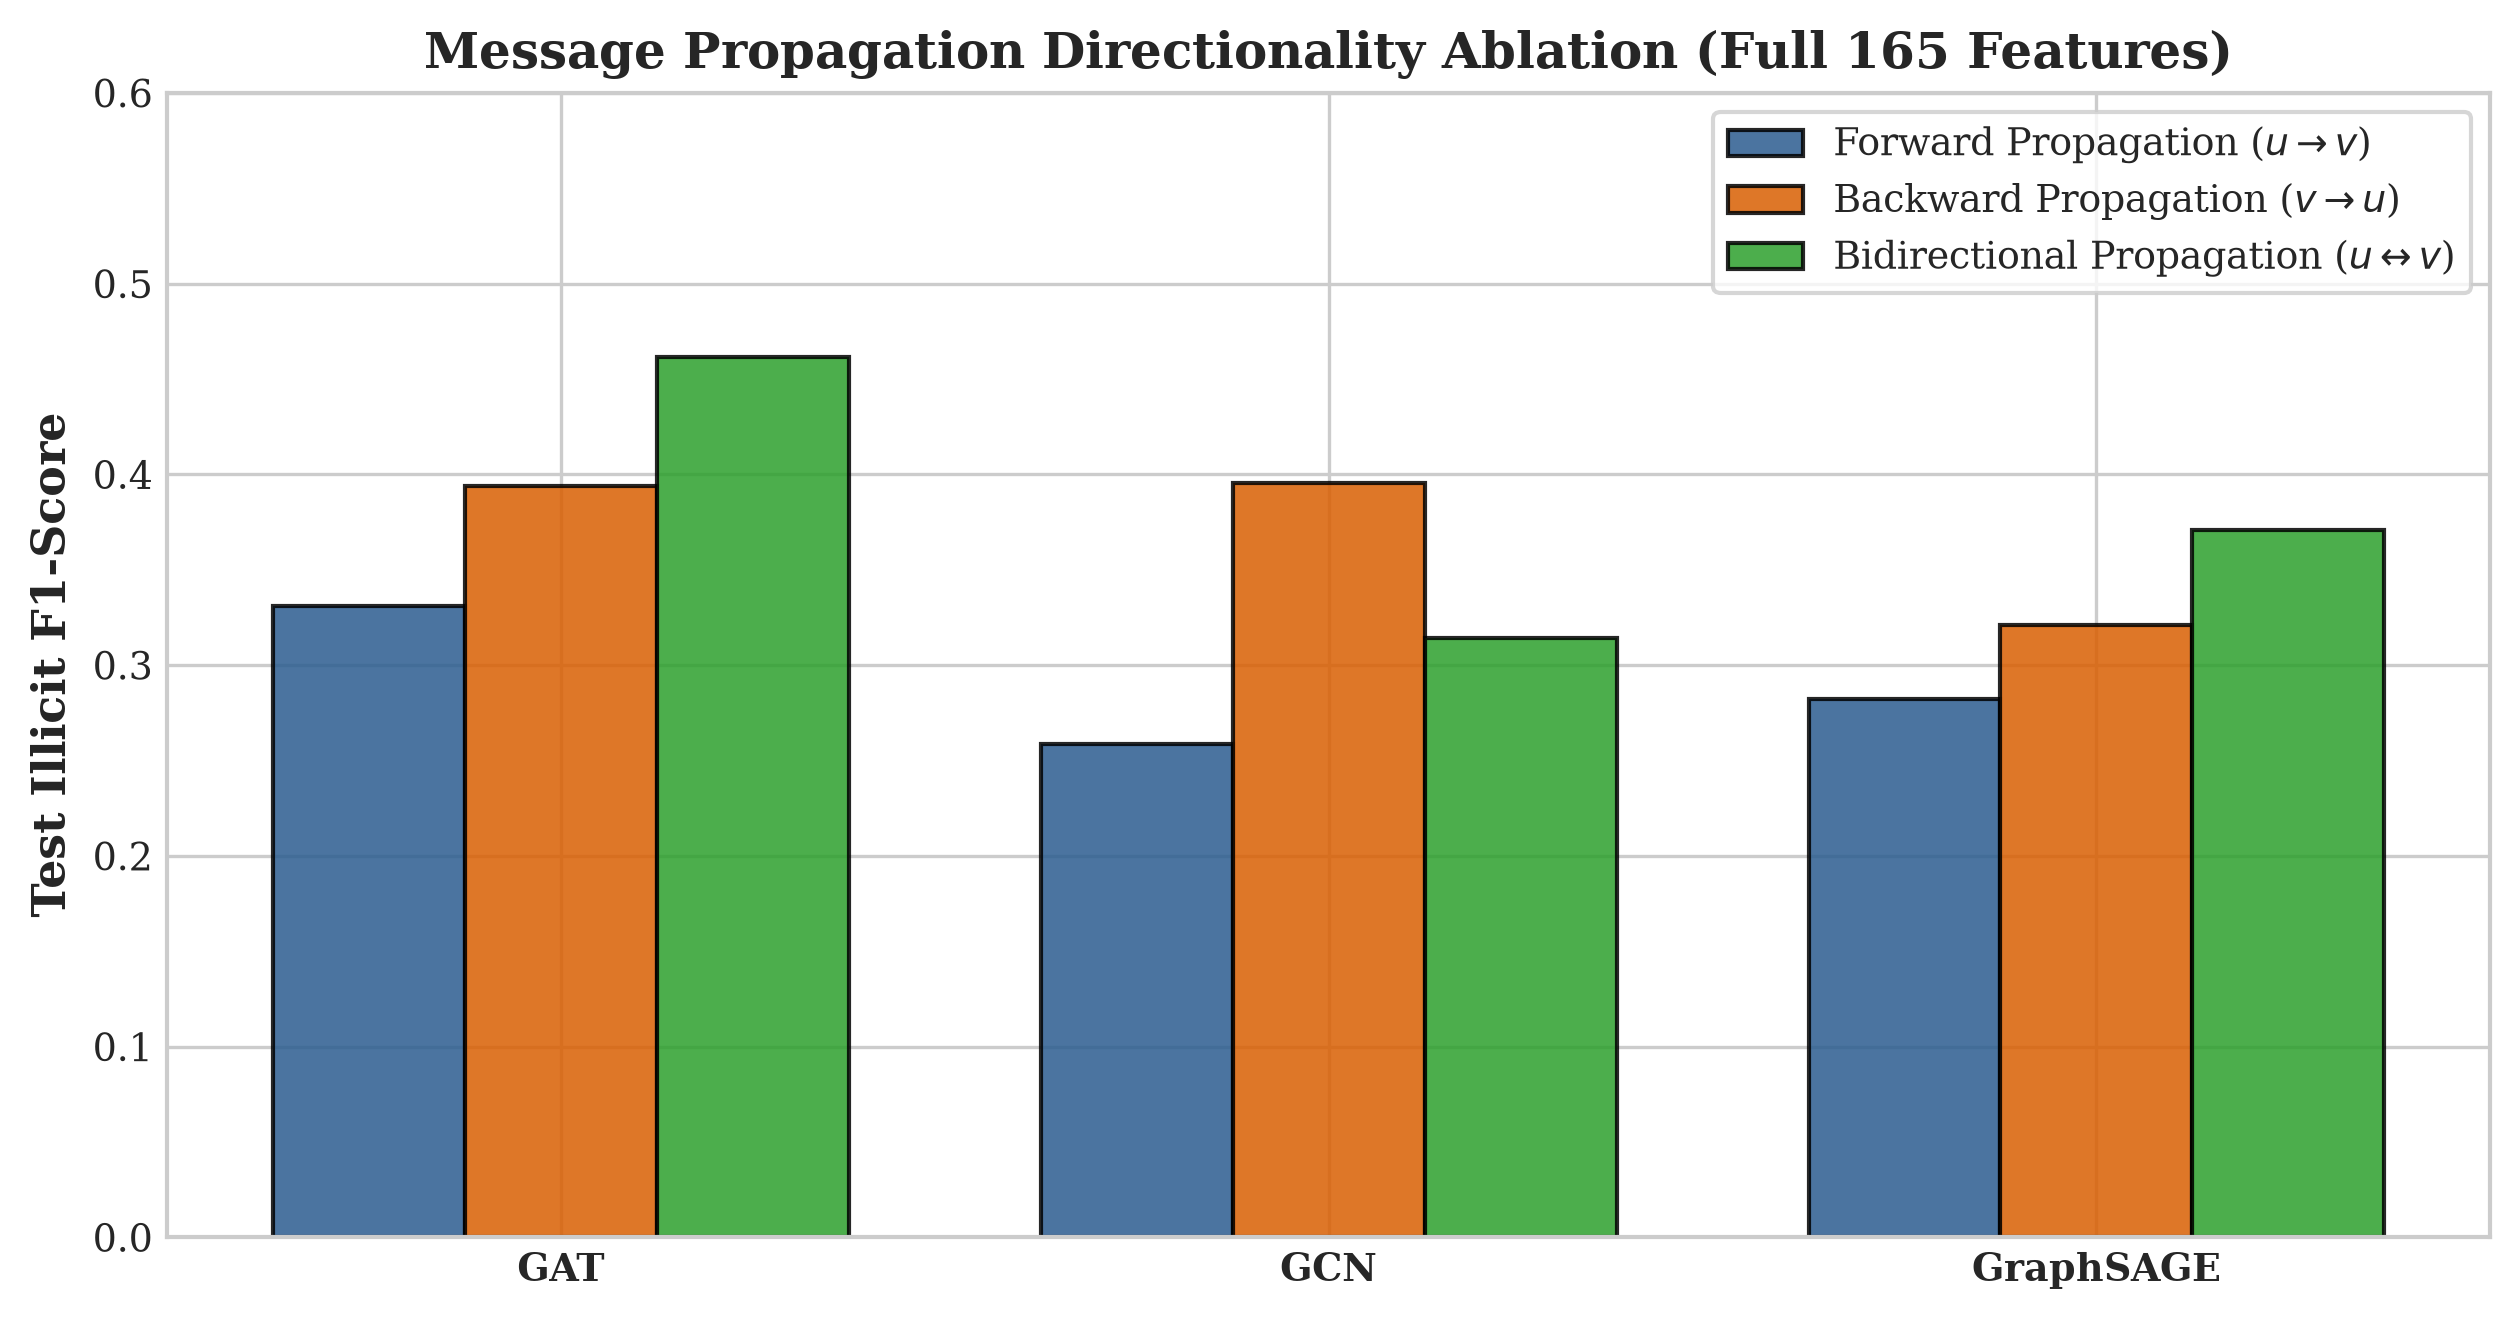
\includegraphics[width=\columnwidth]{../figures/direction_sensitivity_ablation.png}
\caption{Graph directionality ablation comparing Forward, Backward, and Bidirectional message-passing propagation across GNN architectures.}
\label{fig:direction_ablation}
\end{figure}

\subsection{Message-Passing Layer Depth}
Table IX and Fig. 8 show depth responses across 1, 2, and 3 layers:
\begin{itemize}
    \item GCN degraded monotonically ($0.2862 \to 0.2589 \to 0.2089$), consistent with theoretical over-smoothing in isotropic convolutions \cite{li2018deeper, oono2020graph, chen2020measuring}.
    \item GAT peaked at 2 layers ($0.3308 \pm 0.0602$).
    \item GraphSAGE achieved its highest full-feature performance with a single layer ($0.3750 \pm 0.1215$).
\end{itemize}

\begin{table}[htbp]
\centering
\caption{GNN Depth Ablation (Timesteps 40--49, 165 Features)}
\label{tab:depth_ablation}
{\small
\resizebox{\columnwidth}{!}{
\begin{tabular}{lcccc}
\toprule
\textbf{Architecture} & \textbf{1 Layer} & \textbf{2 Layers} & \textbf{3 Layers} & \textbf{Profile} \\
\midrule
GAT & $0.2877 \pm 0.0319$ & $0.3308 \pm 0.0602$ & $0.2847 \pm 0.0052$ & Peak at 2 \\
GCN & $0.2862 \pm 0.0250$ & $0.2589 \pm 0.0639$ & $0.2089 \pm 0.0892$ & Monotonic \\
GraphSAGE & $0.3750 \pm 0.1215$ & $0.2822 \pm 0.1248$ & $0.3327 \pm 0.1250$ & Peak at 1 \\
\bottomrule
\end{tabular}
}
}
\end{table}

\begin{figure}[htbp]
\centering
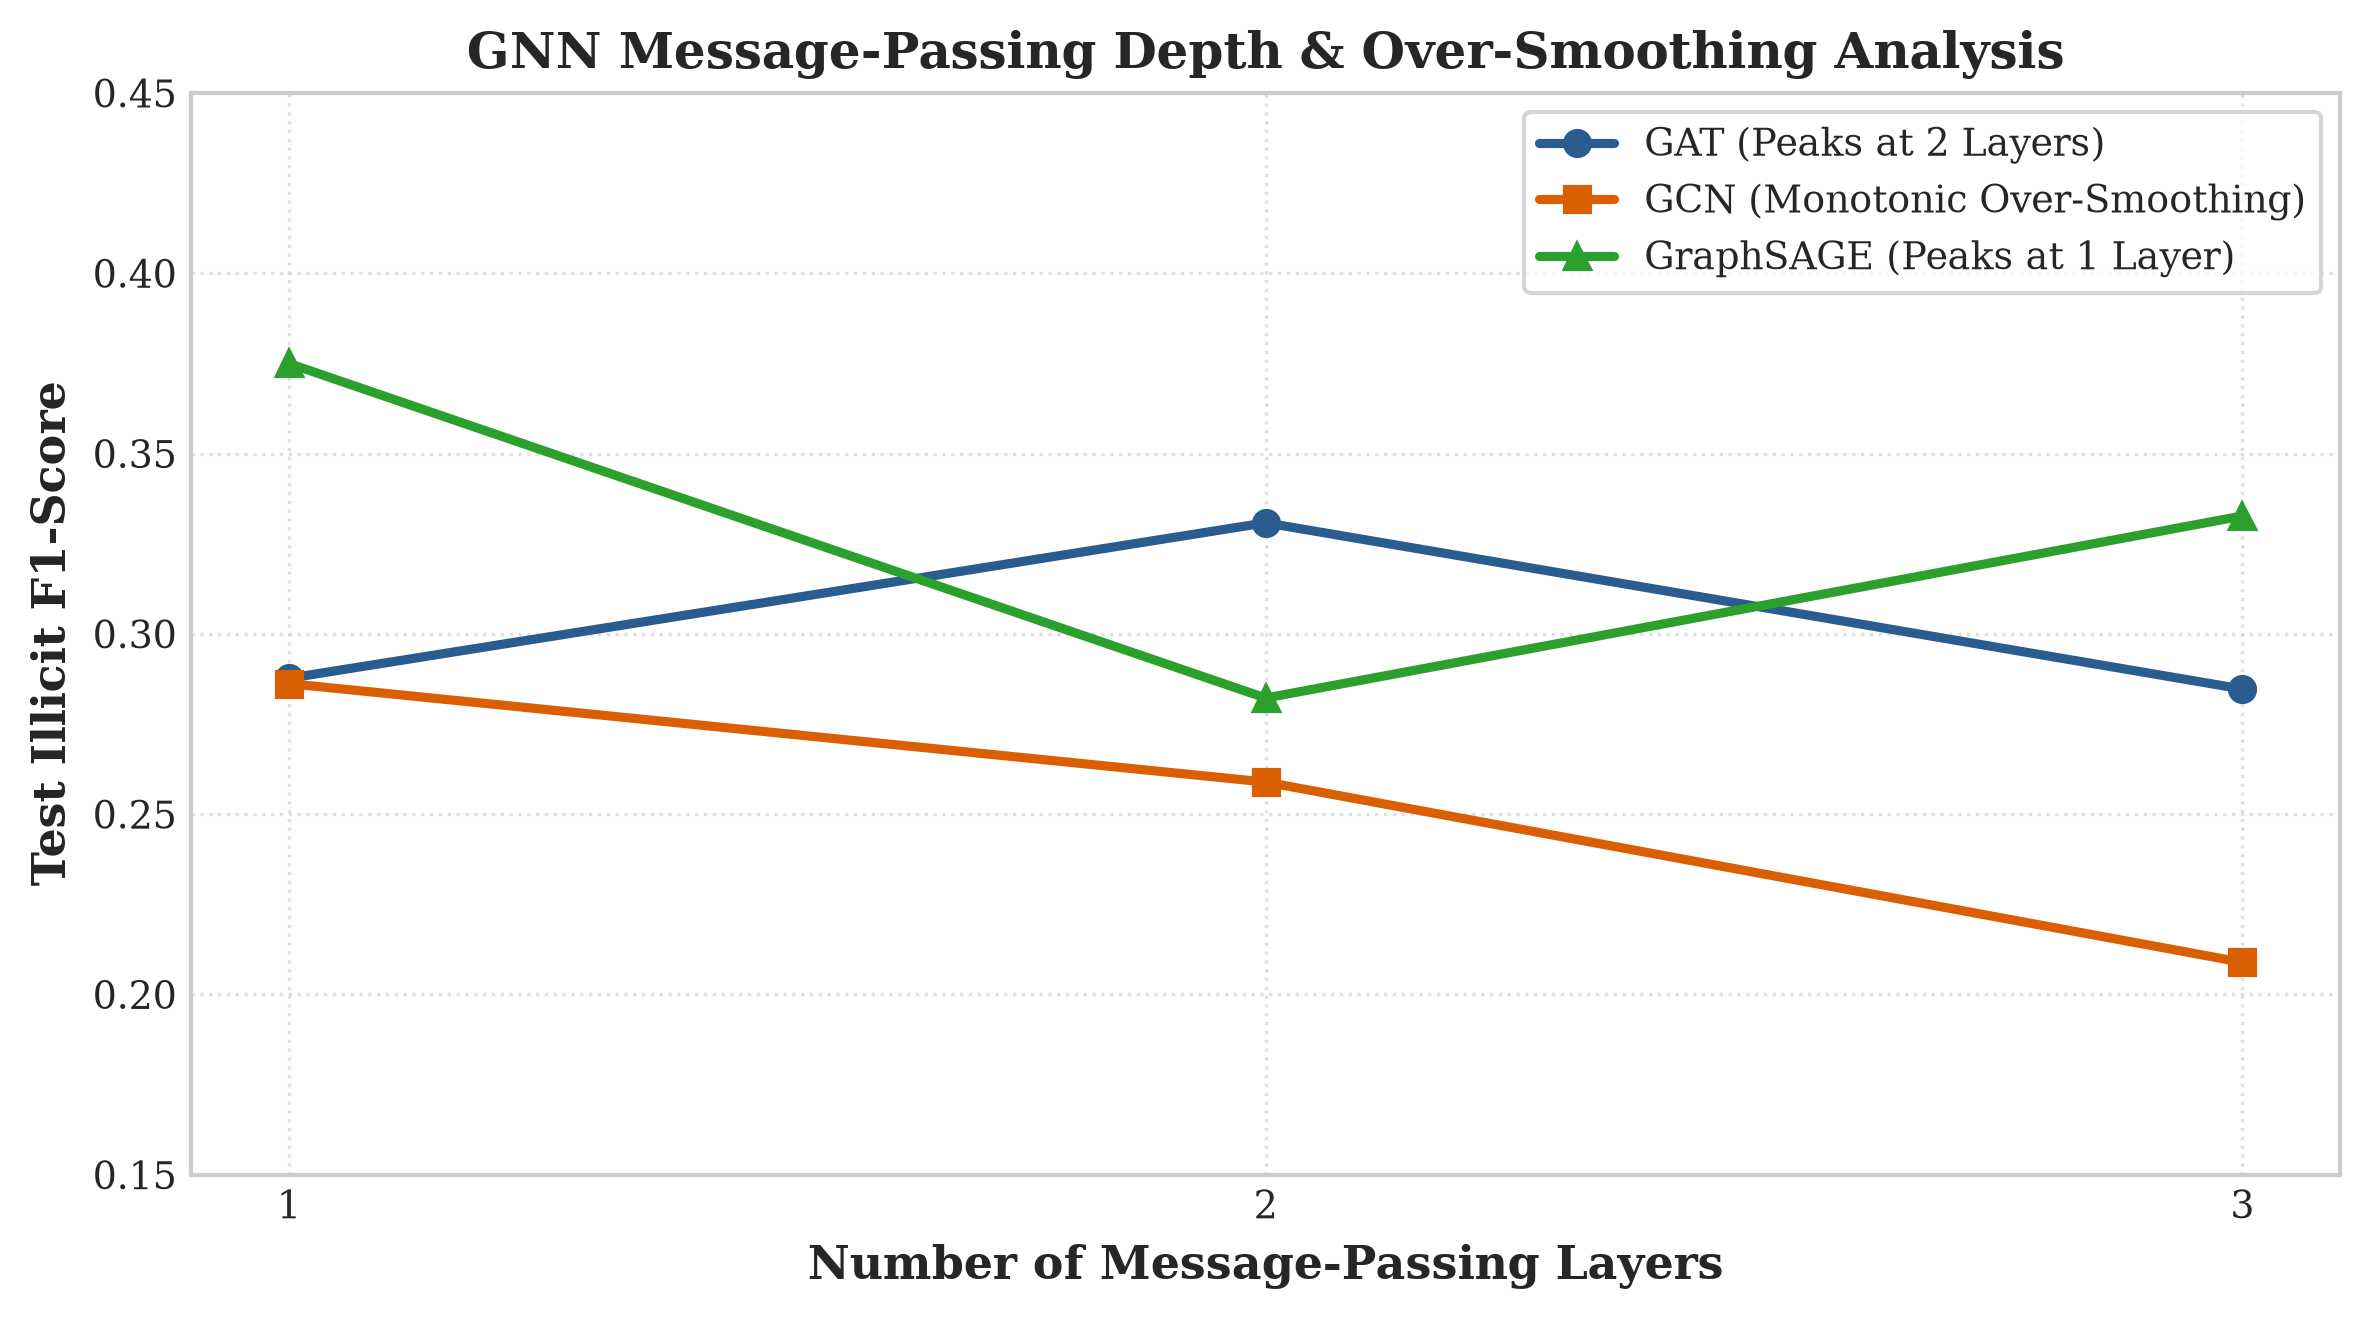
\includegraphics[width=\columnwidth]{../figures/depth_ablation.png}
\caption{Message-passing depth ablation across 1, 2, and 3 layers for GCN, GraphSAGE, and GAT.}
\label{fig:depth_ablation}
\end{figure}

\section{Statistical Analysis}

\subsection{Paired Hypothesis Testing}
To eliminate post-hoc selection bias, we evaluate the validation-selected GNN (\textbf{GraphSAGE on Local 93 Features}, Val F1 $= 0.6060$, Test F1 $= 0.4153 \pm 0.1914$, Test PR-AUC $= 0.3659 \pm 0.1859$) against representative baselines across five shared seeds ($N=5$). As reported in Table X:
\begin{itemize}
    \item Unadjusted paired $t$-tests indicated differences favoring Random Forest ($p_{\text{raw}} = 0.0229$, $d_z = -1.6062$) and XGBoost ($p_{\text{raw}} = 0.0247$, $d_z = -1.5694$) \cite{cohen1988statistical, lakens2013calculating}.
    \item Following Holm-Bonferroni correction \cite{holm1979simple}, adjusted $p$-values increased to $p_{\text{Holm}} = 0.0917$.
    \item Exact paired Wilcoxon signed-rank tests produced $p_{\text{Wilcoxon}} = 0.0625$ \cite{wilcoxon1945individual, demsar2006statistical}.
    \item Consequently, differences do not cross the formal significance threshold of $\alpha = 0.05$ after multiple comparison adjustment.
\end{itemize}

\begin{table*}[t]
\centering
\caption{Paired Statistical Significance Tests (GraphSAGE Local 93 vs. Baselines, $N=5$ Seeds)}
\label{tab:stats_tests}
\begin{tabular}{lcccccccc}
\toprule
\textbf{Metric / Comparison} & \textbf{Mean Diff ($\Delta$)} & \textbf{Paired $t$} & \textbf{$p$ (Raw)} & \textbf{$p$ (Holm)} & \textbf{$W$-Stat} & \textbf{$p$ (Wilcoxon)} & \textbf{Cohen $d_z$} & \textbf{FWER Signif.} \\
\midrule
\textbf{Test Illicit F1} & & & & & & & & \\
vs. Random Forest & $-0.3094$ & $-3.5917$ & $0.0229$ & $0.0917$ & $0.0$ & $0.0625$ & $-1.6062$ & No ($p \ge 0.05$) \\
vs. XGBoost & $-0.3044$ & $-3.5092$ & $0.0247$ & $0.0917$ & $0.0$ & $0.0625$ & $-1.5694$ & No ($p \ge 0.05$) \\
vs. MLP & $-0.1695$ & $-1.8872$ & $0.1322$ & $0.2644$ & $3.0$ & $0.3125$ & $-0.8440$ & No ($p \ge 0.05$) \\
vs. Logistic Regression & $+0.0673$ & $+0.7856$ & $0.4760$ & $0.4760$ & $6.0$ & $0.8125$ & $+0.3513$ & No ($p \ge 0.05$) \\
\midrule
\textbf{Test PR-AUC} & & & & & & & & \\
vs. Random Forest & $-0.2940$ & $-3.5141$ & $0.0246$ & $0.0816$ & $0.0$ & $0.0625$ & $-1.5716$ & No ($p \ge 0.05$) \\
vs. XGBoost & $-0.3064$ & $-3.7246$ & $0.0204$ & $0.0816$ & $0.0$ & $0.0625$ & $-1.6657$ & No ($p \ge 0.05$) \\
vs. MLP & $-0.1456$ & $-1.6440$ & $0.1755$ & $0.3070$ & $3.0$ & $0.3125$ & $-0.7352$ & No ($p \ge 0.05$) \\
vs. Logistic Regression & $+0.1462$ & $+1.7584$ & $0.1535$ & $0.3070$ & $3.0$ & $0.3125$ & $+0.7864$ & No ($p \ge 0.05$) \\
\bottomrule
\end{tabular}
\end{table*}

\subsection{Statistical Power Bounds at $N=5$}
For sample size $N = 5$, there are $2^5 = 32$ possible signed-rank permutations. The minimum achievable two-sided Wilcoxon $p$-value is mathematically bounded at:
\begin{equation}
p_{\min} = \frac{2}{2^5} = \frac{2}{32} = 0.0625
\label{eq:power_bound}
\end{equation}
It is therefore mathematically impossible for a two-sided Wilcoxon test with $N=5$ to achieve $p < 0.05$, regardless of effect magnitude \cite{wilcoxon1945individual, demsar2006statistical}.

\section{Error and Graph-Structural Analysis}

\subsection{Error Taxonomy and Degree Disparity}
Table XI details error distributions and connectivity across the $11,184$ test nodes ($402$ TP, $8,165$ TN, $2,383$ FP, $234$ FN):
\begin{itemize}
    \item True Negatives had the highest connectivity (mean in-degree $2.38$, out-degree $1.34$).
    \item True Positives had the lowest connectivity (mean in-degree $0.87$, out-degree $0.70$).
    \item The test set contained zero high-confidence false positives ($\hat{p} \ge 0.80$) and zero high-confidence false negatives ($\hat{p} \le 0.20$), indicating that misclassifications occurred in regions of model uncertainty.
\end{itemize}

\begin{table}[htbp]
\centering
\caption{Error and Graph-Structural Taxonomy (Test Set, $N = 11,184$)}
\label{tab:error_taxonomy}
{\small
\resizebox{\columnwidth}{!}{
\begin{tabular}{lcccc}
\toprule
\textbf{Category / Segment} & \textbf{Count} & \textbf{Prop. (\%)} & \textbf{In-Deg.} & \textbf{Out-Deg.} \\
\midrule
Total Test Nodes & 11,184 & 100.00\% & 2.06 & 1.26 \\
True Positives (TP) & 402 & 3.59\% & 0.87 & 0.70 \\
True Negatives (TN) & 8,165 & 73.01\% & 2.38 & 1.34 \\
False Positives (FP) & 2,383 & 21.31\% & 1.23 & 1.13 \\
False Negatives (FN) & 234 & 2.09\% & 1.61 & 0.87 \\
High-Confidence FP ($\hat{p} \ge 0.80$) & 0 & 0.00\% & 0.00 & 0.00 \\
High-Confidence FN ($\hat{p} \le 0.20$) & 0 & 0.00\% & 0.00 & 0.00 \\
\bottomrule
\end{tabular}
}
}
\end{table}

\subsection{Graph Homophily and Relational Topology}
Of $234,355$ directed edges, only $36,624$ ($15.63\%$) connect two labeled nodes. Among mutually labeled edges, same-class homophily is $95.37\%$ ($34,928 / 36,624$):
\begin{equation}
h_{\text{labeled}} = \frac{34,928}{36,624} = 95.37\%
\label{eq:homophily}
\end{equation}
Conversely, $197,731$ edges ($84.37\%$) involve at least one unknown node (see Fig. 10).

\begin{figure}[htbp]
\centering
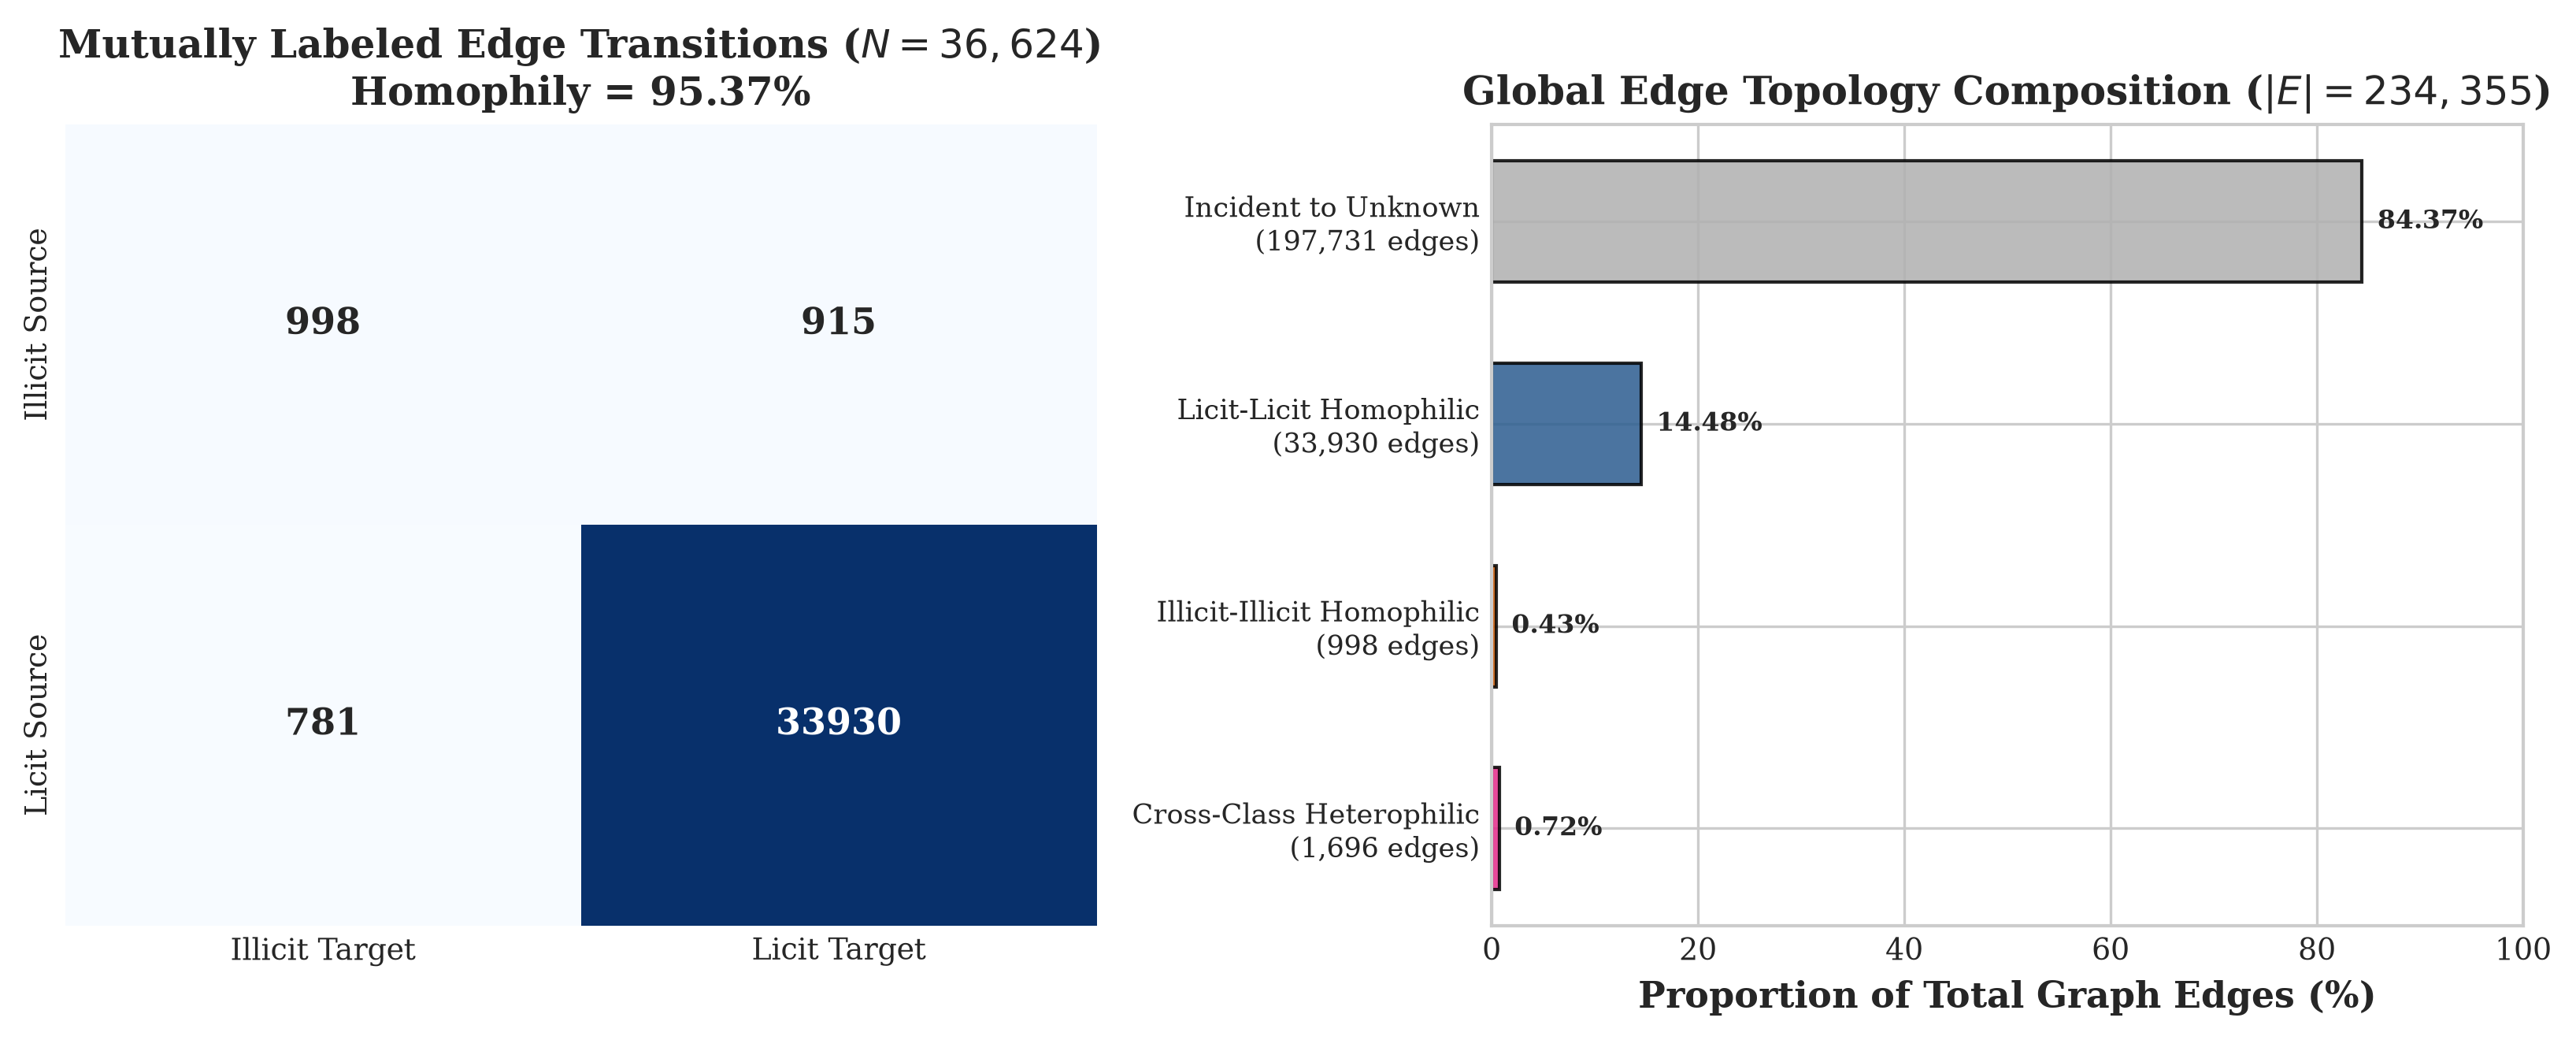
\includegraphics[width=\columnwidth]{../figures/edge_homophily_matrix.png}
\caption{Edge class transition matrix and relational homophily distribution among labeled and unlabeled transaction nodes.}
\label{fig:homophily_matrix}
\end{figure}

\subsection{Temporal Error Patterns across Timesteps 40--49}
Analyzing individual test timesteps (see Fig. 11) reveals that during Timesteps 40--42, illicit prevalence was high ($9.25\%$--$11.10\%$, test F1 up to $0.5234$). At \textbf{Timestep 43}, illicit transaction prevalence collapsed by $84\%$ ($11.10\% \to 1.75\%$), driving test F1 down to $0.0718$.

\begin{figure}[htbp]
\centering
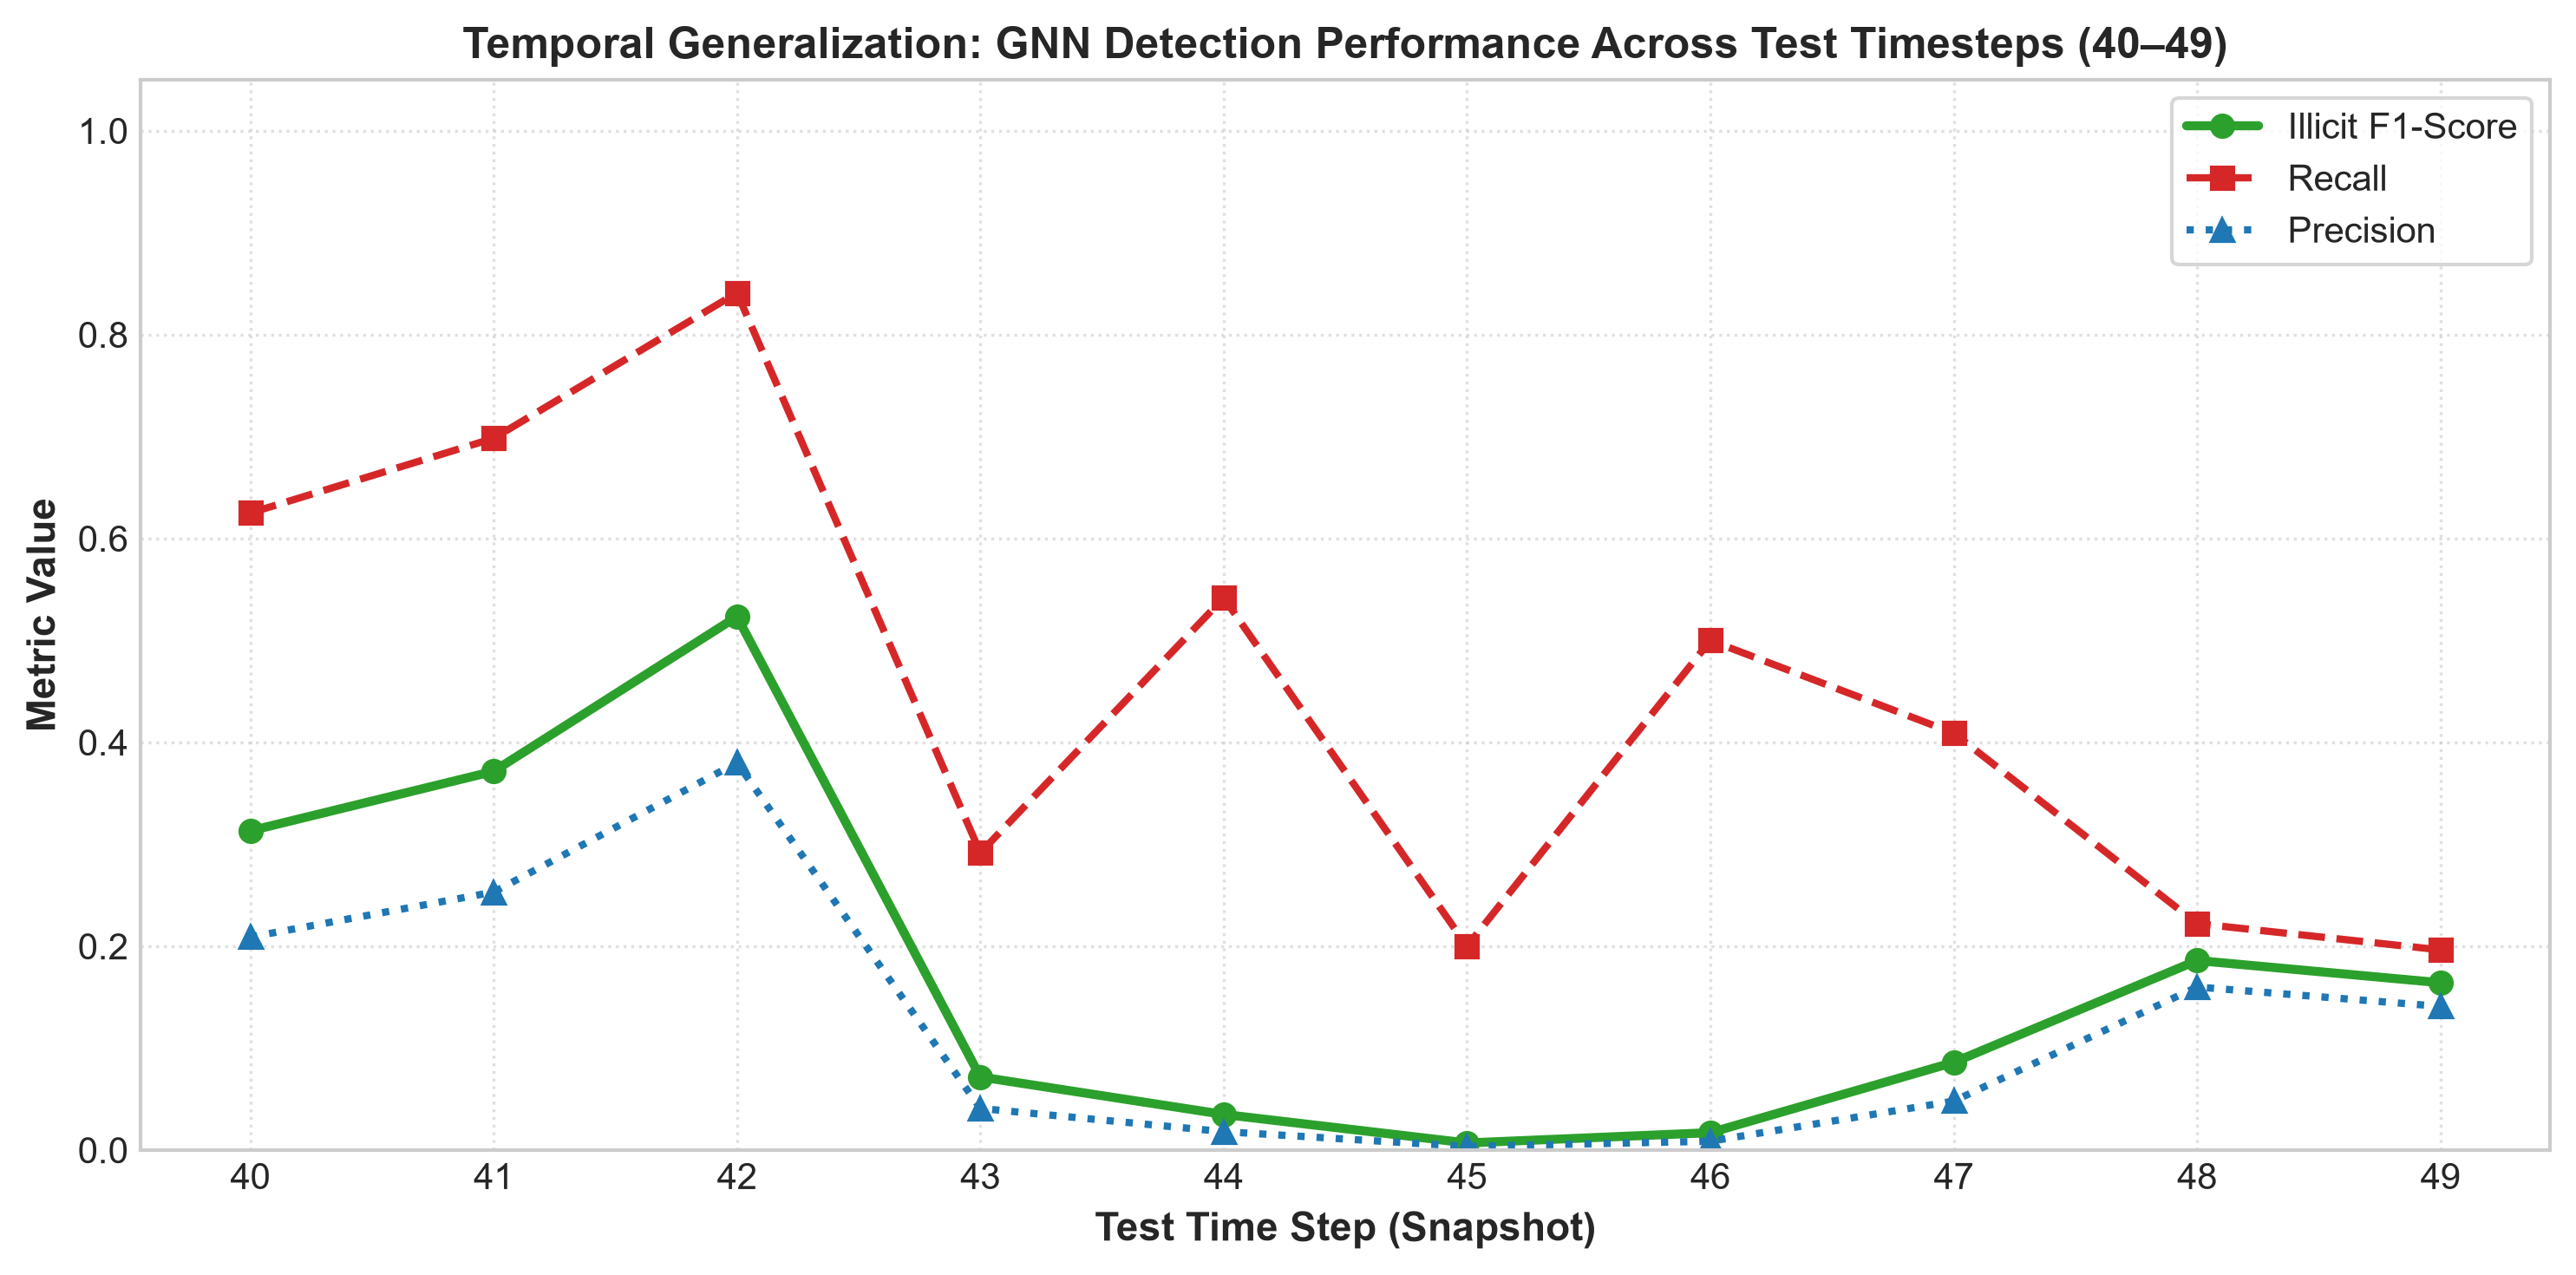
\includegraphics[width=\columnwidth]{../figures/gnn_temporal_performance_timesteps.png}
\caption{Timestep-by-timestep test performance breakdown across timesteps 40–49, illustrating performance collapse during the Timestep 43 regime shift.}
\label{fig:temporal_timesteps}
\end{figure}

\section{Discussion}

\subsection{Comparative Performance of GNNs versus Tabular Baselines}
Under the evaluated chronological protocol, tree-based ensembles (Random Forest F1 $0.7247$, XGBoost F1 $0.7131$) outperformed the evaluated GNN models (GAT $0.3308$, GraphSAGE $0.2822$, GCN $0.2589$) on full features. This outcome is conditional on the benchmark setup and does not constitute universal proof of GNN inferiority \cite{errica2020fair, grinsztajn2022why}.

\subsection{Critical Evaluation of Relational Inductive Bias}
The availability of relational transaction structure does not guarantee that spatial GNNs will outperform strong tabular models \cite{bronstein2017geometric, wang2021graph}. When tabular classifiers receive 1-hop pre-engineered aggregates, decision trees partition feature space orthogonally without propagating raw feature noise across sparse neighborhoods \cite{breiman2001random, chen2016xgboost, grinsztajn2022why}.

\subsection{Feature Representation Dynamics}
Handcrafted 1-hop aggregates improved Random Forest ($+0.0311$ F1), XGBoost ($+0.0430$ F1), MLP ($+0.0187$ F1), and GAT ($+0.0942$ F1), but degraded GraphSAGE ($-0.1331$ F1), indicating architecture-specific feature interactions.

\subsection{Class Imbalance and Threshold Tuning Dynamics}
Because models underwent validation threshold tuning ($\tau^* = \arg\max \text{F1}_{\text{val}}$), unweighted models adjusted decision thresholds effectively. Loss weighting ($w_{\text{pos}} = 7.63$) shifted precision-recall operating trade-offs without offering consistent F1 gains.

\subsection{Temporal Distribution Shift and Concept Drift}
All architectures experienced substantial validation-to-test drops ($23.6\%$ to $44.9\%$), reflecting temporal distribution shift \cite{gama2014survey, quinonero2009dataset}.

\subsection{Seed Sensitivity and Optimization Landscape}
Tree models showed tight cross-seed clustering ($\sigma \le 0.0111$), while GNNs displayed substantial initialization dispersion (GraphSAGE Local range $\Delta = 0.3669$, GCN Full range $\Delta = 0.4686$).

\subsection{Structural Role of Unlabeled Transactions}
GCN and GraphSAGE achieved higher F1 on the isolated labeled subgraph ($0.2589 \to 0.4555$ and $0.2822 \to 0.4132$), whereas GAT performed best when unknown nodes were retained ($0.2918 \to 0.3308$).

\subsection{Causal Directionality versus Retrospective Leakage}
Backward propagation yielded higher retrospective test F1 ($0.3213$--$0.3953$), but relies on future context unavailable during live transaction broadcast; forward flow remains the proper inductive standard.

\subsection{Over-Smoothing and Layer Depth Dynamics}
GCN degraded monotonically with depth ($0.2862 \to 0.2589 \to 0.2089$), consistent with potential over-smoothing across isotropic convolutions \cite{li2018deeper, oono2020graph, chen2020measuring}. GAT peaked at 2 layers ($0.3308$), and GraphSAGE peaked at 1 layer ($0.3750$).

\subsection{Statistical Power and Multiple Comparison Corrections}
While raw paired $t$-tests indicated differences favoring tree ensembles ($p_{\text{raw}} \approx 0.023$), adjusted hypothesis tests did not cross $\alpha = 0.05$ after Holm-Bonferroni correction ($p_{\text{Holm}} = 0.0917$) or Wilcoxon signed-rank testing ($p = 0.0625$) due to small sample power bounds ($N=5$) \cite{wilcoxon1945individual, holm1979simple, demsar2006statistical}.

\subsection{Structural Profiles of Model Misclassifications}
True positives exhibited lower connectivity (mean degree $< 1.0$) than true negatives (mean degree $> 2.0$), indicating that isolated illicit nodes present unique forensic detection challenges.

\subsection{Darknet Market Dynamics and Timestep 43 Non-Stationarity}
The sharp drop in illicit transaction volume at Timestep 43 underscores the vulnerability of static forensic models to sudden macroeconomic and law enforcement interventions \cite{weber2019elliptic, arp2022dos}.

\subsection{Practical Implications for Industry and Regulators}
In production compliance environments, well-tuned gradient boosting ensembles with engineered topological aggregates offer strong detection capability, low inference latency, and high parameter stability.

\begin{table*}[t]
\centering
\caption{Research Question Answer Matrix}
\label{tab:rq_matrix}
\begin{tabular}{p{1.2cm}p{3.5cm}p{4.2cm}p{6.5cm}}
\toprule
\textbf{RQ ID} & \textbf{Core Investigation} & \textbf{Quantitative Finding} & \textbf{Principal Scientific Conclusion} \\
\midrule
\textbf{RQ1} & GNN vs. Tabular Performance & RF F1: $0.7247$, XGB F1: $0.7131$ vs. GAT: $0.3308$, SAGE: $0.2822$, GCN: $0.2589$ & Tree ensembles outperformed GNNs under the evaluated setup; graph convolution did not automatically surpass tabular models. \\
\textbf{RQ2} & Feature Space \& Loss Formulations & 1-Hop Features: $+0.03$ to $+0.04$ for trees, $+0.09$ for GAT, $-0.13$ for SAGE & Aggregated features benefit tree models consistently, while GNN responses are architecture-dependent. \\
\textbf{RQ3} & Topological Context, Direction \& Depth & Unknowns: GCN/SAGE $+0.13$--$+0.20$ without unknowns; GAT $+0.04$ with unknowns & GNN sensitivity to unlabeled context, directionality, and depth is architecture-specific. \\
\textbf{RQ4} & Temporal Shift, Seed Variance \& Errors & Val-to-Test drop: $-23.6\%$ to $-44.9\%$; GNN seed range up to $0.4686$ & Severe temporal non-stationarity and initialization sensitivity impact model reliability. \\
\bottomrule
\end{tabular}
\end{table*}

\section{Limitations}

\subsection{Anonymized Feature Semantics}
Features in the Elliptic benchmark are fully anonymized, precluding domain-specific feature interpretation.

\subsection{High Proportion of Unlabeled Transactions}
$77.15\%$ of transactions lack labels, limiting full relational ground truth.

\subsection{Temporal Non-Stationarity and Regime Shifts}
Adversarial adaptation and darknet market disruptions introduce substantial concept drift \cite{gama2014survey, quinonero2009dataset}.

\subsection{Statistical Power Constraints with Five Seeds}
Evaluating $N=5$ random seeds limits the mathematical power of non-parametric statistical tests ($p_{\min} = 0.0625$).

\subsection{Static Architecture Limitations}
Evaluated GNNs operate on static graph snapshots rather than continuous-time dynamic graphs.

\subsection{Homogeneous Graph Assumptions}
Transactions and payment flows are modeled as homogeneous graphs, omitting heterogeneous entity types \cite{arp2022dos}.

\subsection{Dataset-Specific Generalization Boundaries}
Conclusions are established on the Elliptic Bitcoin dataset and require validation on other blockchain networks.

\subsection{Discrete Temporal Snapshots}
Transactions are aggregated into 2-week snapshots rather than continuous transaction streams.

\section{Conclusion and Future Work}

\subsection{Conclusion}
This study presented a controlled empirical comparison of Graph Neural Networks and conventional tabular machine learning on the Elliptic Bitcoin dataset under chronological partitioning. Tree ensembles (Random Forest and XGBoost) demonstrated strong performance on the full feature representation, benefiting consistently from 1-hop topological aggregates. In contrast, GNN performance proved highly sensitive to graph directionality, unlabeled context, layer depth, and parameter initialization. Spatial graph convolution does not automatically guarantee superiority over well-engineered tabular models in financial transaction forensics.

\subsection{Future Work}
Future research should explore continuous-time dynamic graph neural networks \cite{rossi2020temporal, xu2020inductive}, heterogeneous transaction graphs, and drift-adaptive online learning mechanisms.

\section*{Acknowledgment}
The authors acknowledge the creators of the Elliptic dataset for providing the benchmark data.

\bibliographystyle{IEEEtran}
\bibliography{references}

\end{document}
